\chapter{Lifted Neural Network Training}\label{ch:lifted}

This chapter develops a principled reformulation of neural network training and inversion based on the introduction of auxiliary variables and structured penalties via Bregman distances. Rather than optimising a deeply nested function composition directly through back-propagation, lifted methods ``lift'' the problem into a higher-dimensional space where layer-wise variables are made explicit and controlled through convex penalties. This transformation offers three fundamental advantages: (i) it enables distributed, parallelisable updates that circumvent sequential gradient propagation; (ii) it handles non-smooth activation functions natively without requiring sub-gradient substitutions; and (iii) it provides a unified route to both stable network training and regularised network inversion through the same Bregman framework. We begin with the theoretical foundations and the Bregman penalty framework, proceed to a unified representation of diverse network architectures, discuss optimisation algorithms tailored to lifted objectives, and conclude with concrete applications to inverse problems — specifically, the recovery of network inputs from noisy output observations with provable convergence guarantees.

\section{Foundations of Lifted Training and the Bregman Framework}

We establish the conceptual and mathematical foundations of lifted training by first examining the inherent limitations of standard back-propagation training, then introducing intermediate reformulations such as the Method of Auxiliary Coordinates (MAC) and classical lifted approaches, and finally presenting the lifted Bregman framework — which unifies these ideas through task-dependent penalties based on Bregman distances and proximal operators. This progression reveals how lifted methods address sequential gradient bottlenecks, non-smooth activations, and the degeneracy of naive lifting schemes. The Bregman framework emerges not as an ad-hoc penalty but as a principled Fenchel-Young consistency condition between layer activations and pre-activations, ensuring both convexity in individual variables and improved theoretical properties.

\subsection{Introduction to Standard Training and its Limitations}
Deep neural networks are standardly trained using gradient-based empirical risk minimisation as introduced in Equation \eqref{eq:dnn-empirical-risk-minimisation}. The goal is to determine the optimal network parameters by minimising an objective function across a dataset. For a feed-forward neural network $\mathcal{N}$ parameterised by $\mathbf{\Theta} = \{\Theta_l\}_{l=1}^L$ as defined in \eqref{eq:dnn} and instantiated for multi-layer perceptrons in Section \ref{sec:mlp}, the empirical risk minimisation problem typically reads
\begin{equation*}
    \min_{\mathbf{\Theta}} \, \frac{1}{s}\sum_{i=1}^s \ell(y^i, \mathcal{N}(x^i, \mathbf{\Theta})) \, ,
\end{equation*}
where $s$ denotes the number of training samples, $(x^i, y^i)$ are the input and target pairs, and $\ell$ signifies the loss function. The output of the $L$-th layer represents the network's prediction $\mathcal{N}(x^i, \mathbf{\Theta})$. Such models evaluate intermediate representations through recursive application of affine-linear mappings and non-linear activation functions $\sigma_l$, establishing deeply nested dependencies. 

The prevalent strategy consists of adopting gradient descent as introduced in \eqref{eq:gradient_descent} or its stochastic variants, reliant on the well-known back-propagation algorithm to compute the parameter updates (cf. Algorithm \ref{alg:back-prop}). Despite remaining highly effective, back-propagation exhibits notable inherent limitations. Firstly, its strictly sequential nature propagates errors layer-by-layer backwards through the chain rule, creating fundamental bottlenecks for large-scale parallelisation. Secondly, back-propagation can suffer from vanishing or exploding gradients, where weight updates become infinitesimally small or numerically unstable, especially in earlier layers. Furthermore, non-smooth activation functions such as the Rectified Linear Unit (ReLU) inevitably require sub-gradient substitutions, compromising robust convergence rates compared to proximal minimisation approaches. 

\subsection{Distributed Optimisation \& The Method of Auxiliary Coordinates}
To circumvent the sequential nature of gradients, we can reformulate the learning process by introducing auxiliary variables that decouple the network layers. By defining $x_l^i$ as the post-activation state of the $l$-th layer for sample $i$, and keeping the layer transformation denoted as $f(x_{l-1}^i, \Theta_l)$, we constrain the variables to satisfy the forward pass exactly, similar to Equation \eqref{eq:dnn-empirical-risk-minimisation-v2}. This transforms the unconstrained, deeply nested formulation into an equivalent constrained optimisation problem, which reads
\begin{align}
    \begin{split}
    \min_{\mathbf{\Theta}, \mathbf{X}} \, &\frac{1}{s}\sum_{i=1}^s \ell(y^i, x_L^i) \\
    \text{s.t.} \quad &x_l^i = \sigma_l(f(x_{l-1}^i, \Theta_l)) \quad \text{for } l = 1, \ldots, L \, .
    \end{split}\label{eq:constrained_lifted_formulation}
\end{align}
Relaxing these hard architectural constraints yields optimisation strategies that decouple the individual layers. A prominent strategy is the Method of Auxiliary Coordinates (MAC) \cite{CarreiraPerpinan2014}. MAC replaces the equality constraints with quadratic penalty terms. The resulting unconstrained objective reads
\begin{equation}\label{eq:mac_qp}
    \min_{\mathbf{\Theta}, \mathbf{X}} \frac{1}{s} \sum_{i=1}^{s} \left[ \ell(y^i, f(x_{L - 1}^i, \Theta_L)) + \sum_{l=1}^{L-1} \lambda_l \|x^i_{l} - \sigma_l(f(x_{l - 1}^i, \Theta_l)) \|_2^2 \right] \, ,
\end{equation}
with penalty parameters $\lambda_l > 0$. This formulation decomposes the training problem into a series of shallow, loosely coupled sub-problems. Consequently, block-coordinate descent methods can be deployed, distributing the workload across parameter groups spanning multiple layers and data points in parallel. Nonetheless, minimising the MAC objective with gradient-driven routines still enforces the differentiation of the possibly non-smooth activation function $\sigma_l$. 

\subsection{A lifted training approach}\label{sec:lifted}

The second line of work to approach \eqref{eq:constrained_lifted_formulation} is motivated by the observation that the ReLU activation function $\sigma(z, 0) = \max(z, 0)$ itself can be viewed as the solution to a constrained minimisation problem. More specifically, in the work of \cite{zhang2017convergence}, the authors characterise the activated output of the ReLU activation function $\sigma_l (W_l^\top x_{l-1} + b_{l})$ as
\begin{align*}
    x_{l} &= \sigma_l (W_l^\top x_{l-1} + b_{l}) \\
    &= \argmin_{x \geq 0} \|x - (W_l^\top x_{l-1} + b_{l})\|_2^2 \,\, .
\end{align*}
This implies that $x_l$ is the vector closest to $W_l^\top x_{l-1} + b_{l}$ that lies in the non-negative orthant.

\noindent In the classical lifted approach \cite{askari2018lifted}, \eqref{eq:constrained_lifted_formulation} is consequently approximated with
\begin{equation}\label{eq:mlp-classical-lifted-network-training}
    \min_{\mathbf{\Theta},\{x_l^{i} \in \mathbb{R}_{+}^{n}\}_{l=1}^{L-1}} \frac{1}{s} \sum_{i=1}^{s} \left[ \ell(y^i, f(x^{i}_{L-1},\Theta_{L})) + \sum_{l=1}^{L-1} \|x^i_{l} - f(x^{i}_{l-1},\Theta_{l})\|_2^2 \right] \, ,
\end{equation}
where $\{x_l^{i} \in \mathbb{R}_{+}^{n} \}_{l=1}^{L-1}$ denotes that the activation variables across layers $l=1, \ldots, L-1$ for each sample $i$ lie in the non-negative orthant, i.e.\ $\mathbb{R}_{+}^{n} := \{v \in \mathbb{R}^n \,| v_j \geq 0, \; \forall \, j \in \{1 \ldots n\} \}$. This approach is often referred to as the ``lifted'' approach because the search space for network parameters is lifted to become a higher dimensional space that now also includes auxiliary variables. However, this ``lifting'' is obviously also present in MAC-QP.

Even though the overall learning problem \eqref{eq:mlp-classical-lifted-network-training} is not convex, each sub-problem is convex in each individual variable when keeping all other variables fixed. Individual updates are also relatively easy to compute using orthogonal projections onto the non-negative orthant. In terms of distributing the computation of parameters, this approach also enjoys the same benefits that the MAC-QP scheme enjoys.
However, one major limitation that this approach suffers from is that it does not solve the original Problem \eqref{eq:dnn-empirical-risk-minimisation}, but essentially trains an affine-linear network (cf.\ \cite{zach2019contrastive}). This restriction can be shown by examining the optimality system. Consider the case with $s=1$ and one single training sample pair $(x,y)$, then the optimality condition of \eqref{eq:mlp-classical-lifted-network-training} with respect to parameters $b_l$ reads
\begin{equation}\label{eq:optimality_condition_lifted_approach}
   (W_{l}^{\top} x_{l-1} + b_{l} - x_{l}) = 0 \qquad \Longrightarrow \qquad x_{l} = W_{l}^{\top} x_{l-1} + b_{l} \,\,.
\end{equation}
Despite this major limitation, this approach has been considered for computing initialisations of network parameters for other optimisation algorithms \cite{li2019lifted,zach2019contrastive}.

\subsection{The Lifted Bregman Framework}
To circumvent the differentiation of non-smooth activation functions whilst fully maintaining distributed optimisation benefits, we transition the penalty framework towards tailored Bregman distances. This framework mandates that activation functions be proximal maps (Definition~\ref{def:prox_operator}) of proper, convex and lower semi-continuous functions $\Psi$, ensuring
\begin{equation}\label{eq:proximal_activation}
    \sigma_l(z) = \operatorname{prox}_{\Psi}(z) = \argmin_{u} \left\{ \frac{1}{2} \| u - z \|_2^2 + \Psi(u) \right\} \, .
\end{equation}
By Fermat's rule (Theorem~\ref{thm:fermat}), this implies $z - \sigma_l(z) \in \partial \Psi(\sigma_l(z))$, where $\partial \Psi$ denotes the subdifferential of $\Psi$ (Definition~\ref{defi:subdiff}). Rather than the classical lifted penalty of Section~\ref{sec:lifted} -- which, as shown in \eqref{eq:optimality_condition_lifted_approach}, degenerates to an affine-linear network at optimality -- we instead introduce a penalty that vanishes to zero precisely when the proximal constraint is satisfied. Using the Fenchel conjugate (Definition~\ref{def:convex_conjugate}), we define the \emph{Bregman loss} $B_{\Psi}(x, z)$ (cf. \cite{WangBenning2023}) as
\begin{equation}\label{eq:bregman_loss}
    B_{\Psi}(x, z) := \frac{1}{2}\|x\|_2^2 + \Psi(x) + \left(\frac{1}{2}\|\cdot\|_2^2 + \Psi\right)^*(z) - \langle x, z \rangle \, .
\end{equation}
This expression is a direct Fenchel-Young gap for the energy $\Phi := \frac{1}{2}\|\cdot\|_2^2 + \Psi$, i.e.\
\begin{equation}\label{eq:bregman_fenchel_young_gap}
    B_{\Psi}(x, z) = \Phi(x) + \Phi^*(z) - \langle x, z \rangle \ge 0
\end{equation}
by the Fenchel-Young inequality \eqref{eq:fenchel-young}, with equality if and only if $z \in \partial \Phi(x)$. Incorporating $B_{\Psi}$ into the MAC-QP framework \eqref{eq:mac_qp} by replacing the quadratic penalties with the Bregman loss penalties yields the \emph{Lifted Bregman} training problem \cite{WangBenning2023}
\begin{equation}\label{eq:bregman_lifted}
    \min_{\mathbf{\Theta}, \mathbf{X}}  \sum_{i=1}^{s} \left[\ell\left(y^i, x_{L}^{i}\right) + \sum_{l=1}^{L-1} \,  \lambda_l B_{\Psi_l}\left(x_{l}^{i}, f(x_{l - 1}^{i}, \Theta_l) \right)\right] \, .
\end{equation}
Because $B_\Psi$ is \emph{bi-convex} -- convex in $x$ for fixed $z$, and convex in $z$ for fixed $x$ -- each block subproblem arising in a Block-Coordinate Descent (BCD) scheme applied to \eqref{eq:bregman_lifted} is a convex optimisation problem, which directly justifies the distributed layer-by-layer update strategy discussed in Section~\ref{sec:lifted}.

The lifted Bregman penalty can be interpreted as a layer-wise Fenchel-Young consistency loss between activation variables and transformed pre-activations. This directly mirrors the Fenchel-Young parameter-learning viewpoint developed in Chapter~\ref{ch:data-driven}, where the scalar objective $G(\lambda)$ in \eqref{eq:fenchel-young-reg-param} is used to learn regularisation scales and is connected to bilevel training formulations in \eqref{eq:bilevel_upper} -- \eqref{eq:bilevel_lower} and \eqref{eq:scale_upper} -- \eqref{eq:scale_lower}. In this sense, \eqref{eq:bregman_lifted} can be viewed as the network-level analogue of those variational learning objectives: the same Fenchel-Young machinery is now applied to every layer and every sample.
The term \eqref{eq:bregman_loss} is a generalised Bregman distance in the sense of Definition~\ref{defi:bregman}. It satisfies $B_{\Psi}(x,z) \geq 0$ for all $x, z$, with equality if and only if $x = \operatorname{prox}_{\Psi}(z)$, i.e.\ precisely when the proximal architectural constraint is met. Moreover, one can decompose $B_\Psi$ as
\begin{equation}\label{eq:bregman_loss_decomposition}
    B_{\Psi}(x, z) = \frac{1}{2}\|x - \sigma(z)\|_2^2 + D_{\Psi}^{z - \sigma(z)}\!\left(x,\, \sigma(z)\right) \;\geq\; \frac{1}{2}\|x - \sigma(z)\|_2^2 \, ,
\end{equation}
where $D_{\Psi}^{z-\sigma(z)}(x, \sigma(z))$ is the Bregman distance of $\Psi$ (Definition~\ref{defi:bregman}) with subgradient $z - \sigma(z) \in \partial\Psi(\sigma(z))$. The Bregman loss therefore penalises both the distance of $x$ to the proximal point $\sigma(z)$ and the degree to which the activation structure encoded by $\Psi$ is violated, providing a strictly richer penalty than the quadratic term used in \eqref{eq:mac_qp} or \eqref{eq:mlp-classical-lifted-network-training}.

A further critical property is the gradient of $B_\Psi$ with respect to its second argument. By differentiating the Fenchel conjugate and invoking the Moreau decomposition (Theorem~\ref{thm:moreau_decomposition}), one obtains (cf. \cite{WangBenning2023})
\begin{equation}\label{eq:bregman_loss_gradient}
    \nabla_z B_{\Psi}(x, z) = \sigma(z) - x \, .
\end{equation}
This means that updating the network parameters $\Theta_l$ requires only the evaluation of $\sigma_l$, never its derivative, making the framework naturally applicable to non-smooth activations without any sub-gradient approximation.

\begin{exm}[Bregman losses for common activation functions]\normalfont
We give explicit formulae for $B_\Psi$ for three standard proximal activations from \cite{WangBenning2023}.

\noindent \textbf{ReLU.} For $\Psi(u) = \chi_{[0,\infty)^n}(u)$ (the indicator of the non-negative orthant), so that $\sigma(z)_j = \max(z_j, 0)$, we get
\begin{align*}
    B_{\Psi}(x, z) = \begin{cases} \dfrac{1}{2}\|x - \max(z, 0)\|_2^2 + \langle x,\, \max(-z, 0)\rangle & x \in [0,\infty)^n , \\[4pt] \infty & \text{otherwise.} \end{cases}
\end{align*}
Compared to the quadratic penalty used in \eqref{eq:mlp-classical-lifted-network-training}, the additional term $\langle x, \max(-z, 0)\rangle \geq 0$ penalises configurations where $z$ has negative components, and it is precisely its presence that prevents the affine degeneracy of \eqref{eq:optimality_condition_lifted_approach}.

\noindent \textbf{Soft-thresholding.} For $\Psi(u) = \alpha |u |_1$ with $\alpha > 0$, in the scalar case $x, z \in \mathbb{R}$, we observe
\begin{align*}
    B_{\Psi}(x, z) = \begin{cases} \dfrac{1}{2}z^2 - z(\alpha + x) & z > \alpha , \\[4pt] -xz & |z| \leq \alpha , \\[4pt] \dfrac{1}{2}z^2 + z(\alpha - x) & z < -\alpha . \end{cases}
\end{align*}

\noindent \textbf{Hyperbolic tangent.} For $\Psi$ chosen such that $\sigma(z) = \tanh(z)$, in the scalar case $x, z \in \mathbb{R}$, we obtain
\begin{align*}
    B_{\Psi}(x, z) = \begin{cases} \dfrac{1}{2}\log\!\left(\dfrac{1 - x^2}{1 - \tanh^2(z)}\right) + x\bigl(\tanh^{-1}(x) - z\bigr) & |x| < 1 , \\[4pt] \infty & \text{otherwise.} \end{cases}
\end{align*}
\end{exm}

\noindent We visually compare these Bregman losses with their squared Euclidean counterparts in Figure~\ref{fig:bregman_loss_comparisons}.
\begin{figure}[ht]
    \centering
    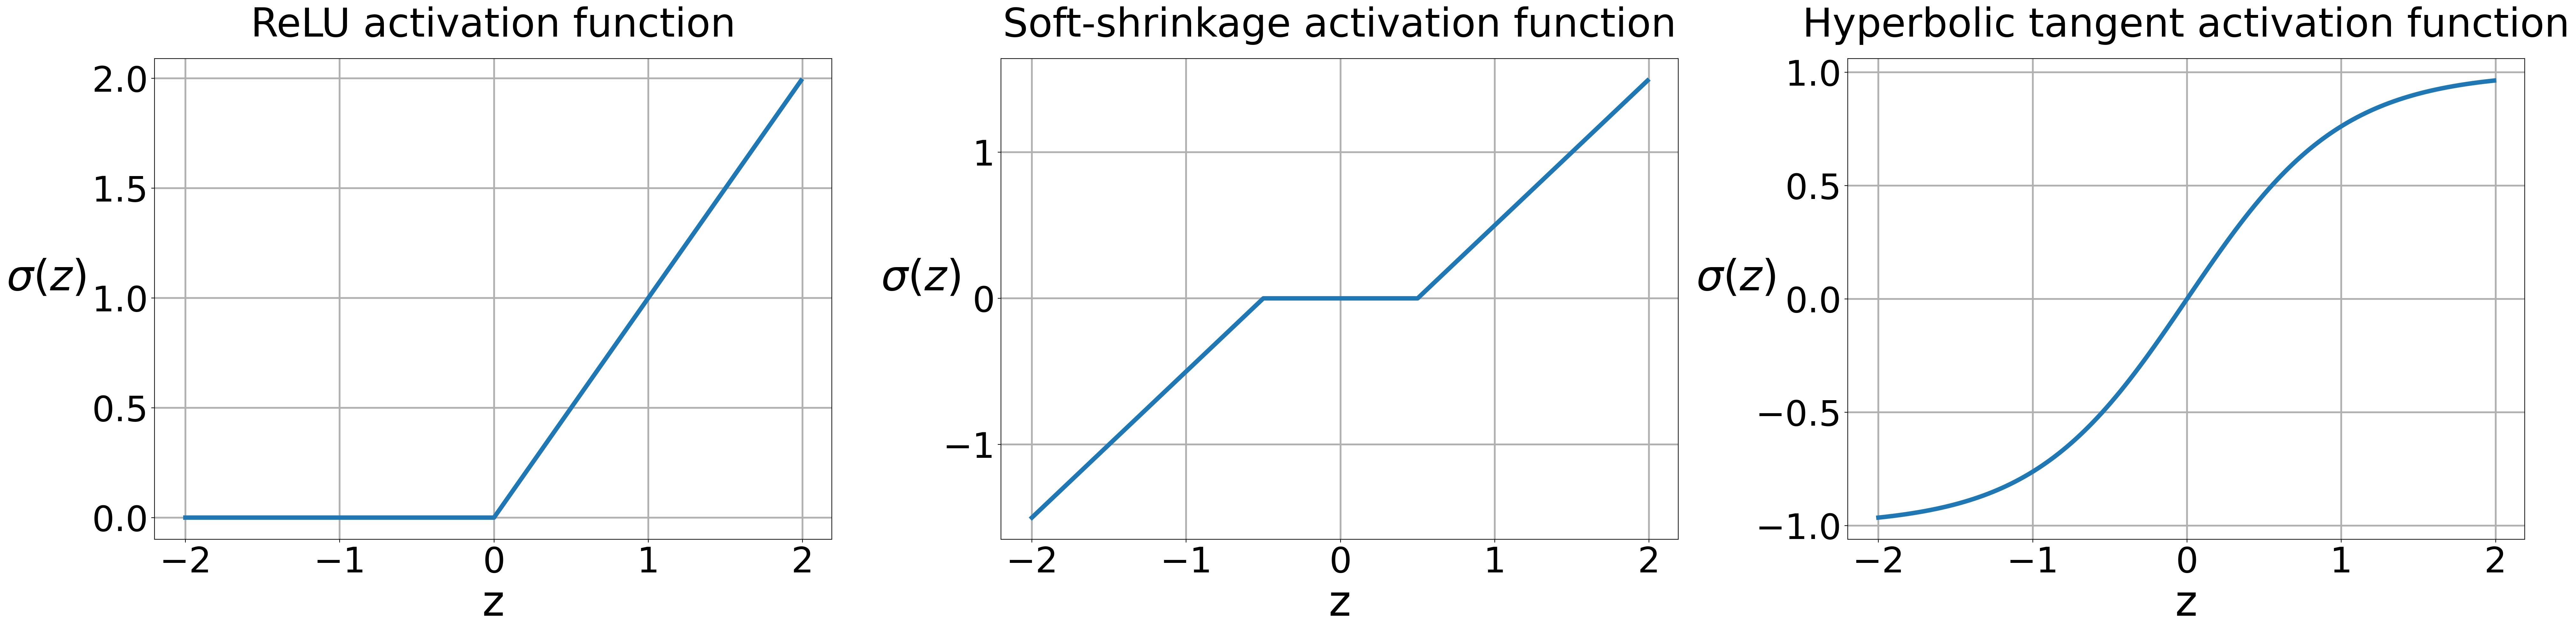
\includegraphics[width=\textwidth]{../Common_Images/lifted/all_three_activation_functions_bigger_font.png}
    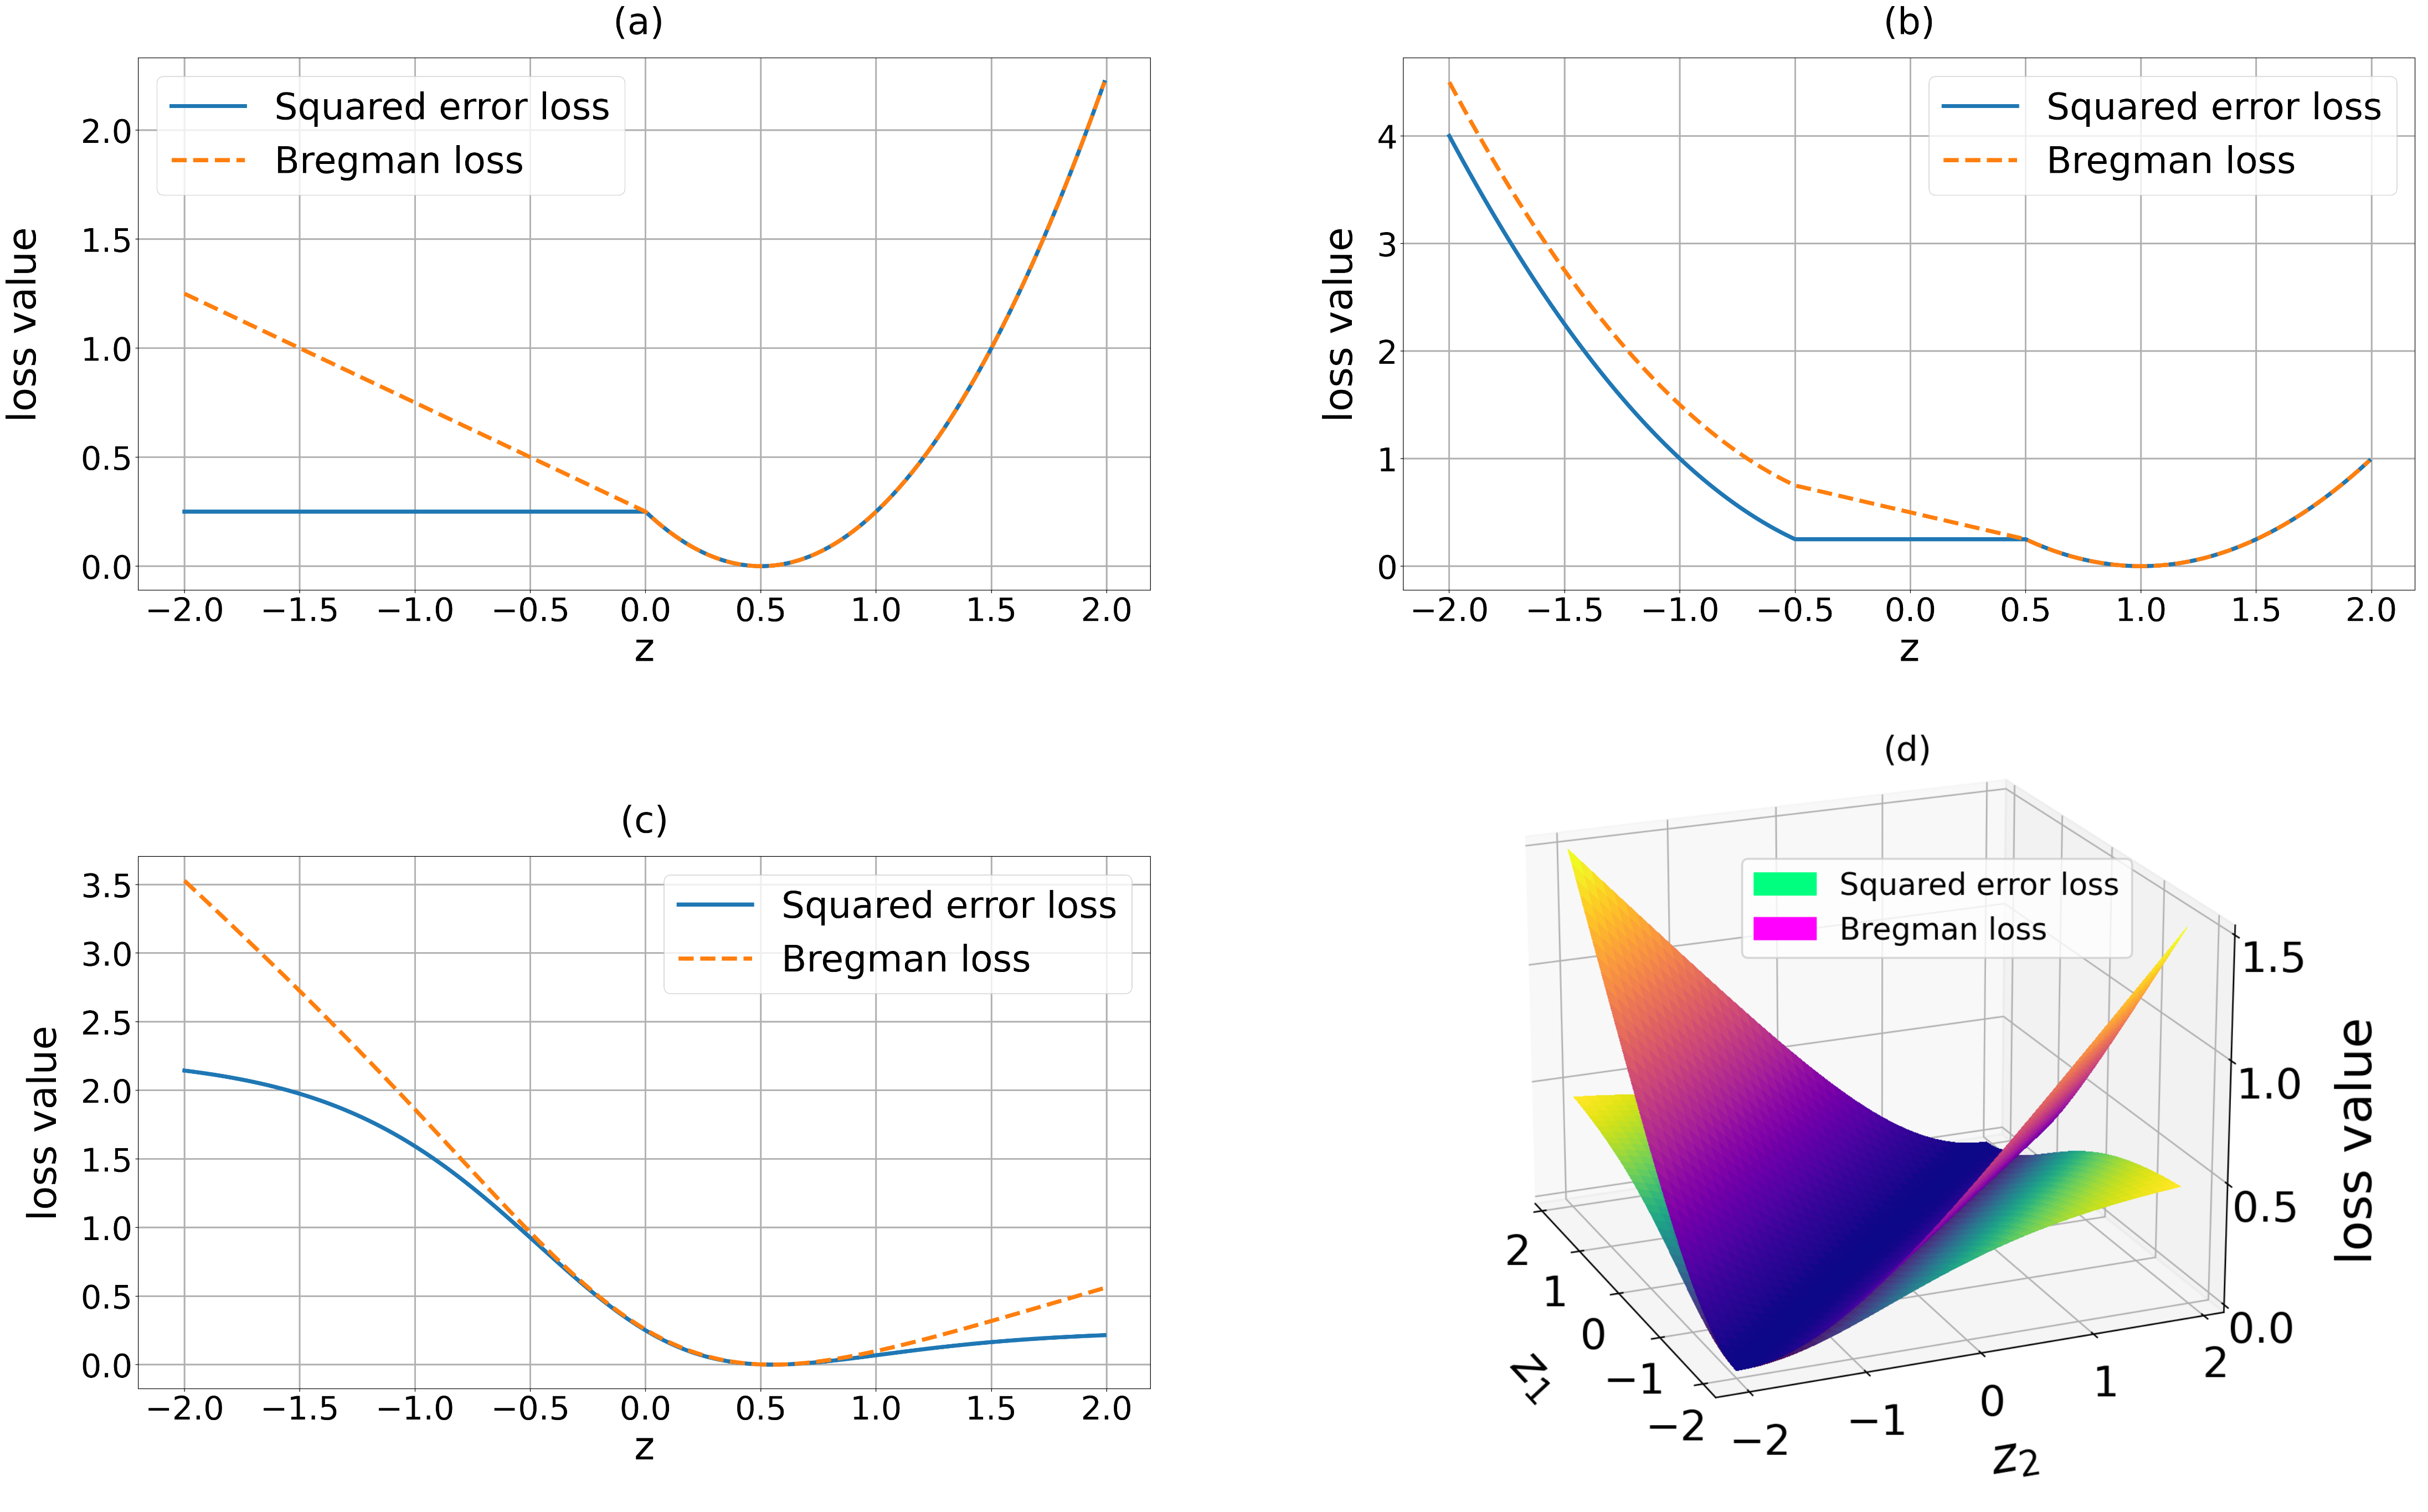
\includegraphics[width=\textwidth]{../Common_Images/lifted/Bregman_loss_plots_bigger_font.png}
    \caption{Top: Different choices of proximal activation functions: ReLU, soft-thresholding, and hyperbolic tangent. Bottom: The associated Bregman losses compared to standard quadratic errors surrounding a target value. The lifted Bregman framework accommodates all mapped characteristics natively.}
    \label{fig:bregman_loss_comparisons}
\end{figure}

\noindent To provide a concrete numerical training example, consider a lifted sparse autoencoder with even depth $L$ and code layer index $m:=L/2$. For inputs $x_0^i$, the decoder output is $x_L^i$, and sparsity is enforced directly on the code variable $x_m^i$. A representative lifted Bregman objective is
\begin{equation}\label{eq:ch9_sparse_autoencoder_objective}
    \min_{\mathbf{\Theta},\mathbf{X}}\; \frac{1}{s}\sum_{i=1}^{s} \left[ \frac12\|x_0^i-x_L^i\|_2^2 + \alpha\|x_m^i\|_1 + \sum_{l=1}^{L-1} \lambda_l B_{\Psi_l}\!\left(x_l^i, f(x_{l-1}^i,\Theta_l)\right) \right] \, .
\end{equation}
Here the first term is the reconstruction loss, the second term promotes sparse latent codes, and the Bregman terms enforce layer-wise proximal consistency. For sparse \emph{denoising} autoencoders, one replaces clean inputs in the encoder by corrupted samples $\tilde x_0^i$ while reconstructing the clean target $x_0^i$. Based on this, a representative numerical snapshot from \cite{WangBenning2023} is shown in Figure~\ref{fig:lifted_bregman_numerical_snapshot}. The plots illustrate that lifted Bregman training can rapidly reduce the sparse-autoencoder objective while sustaining high code sparsity, and can still produce high-quality reconstructions on validation data.
\begin{figure}[ht]
    \centering
    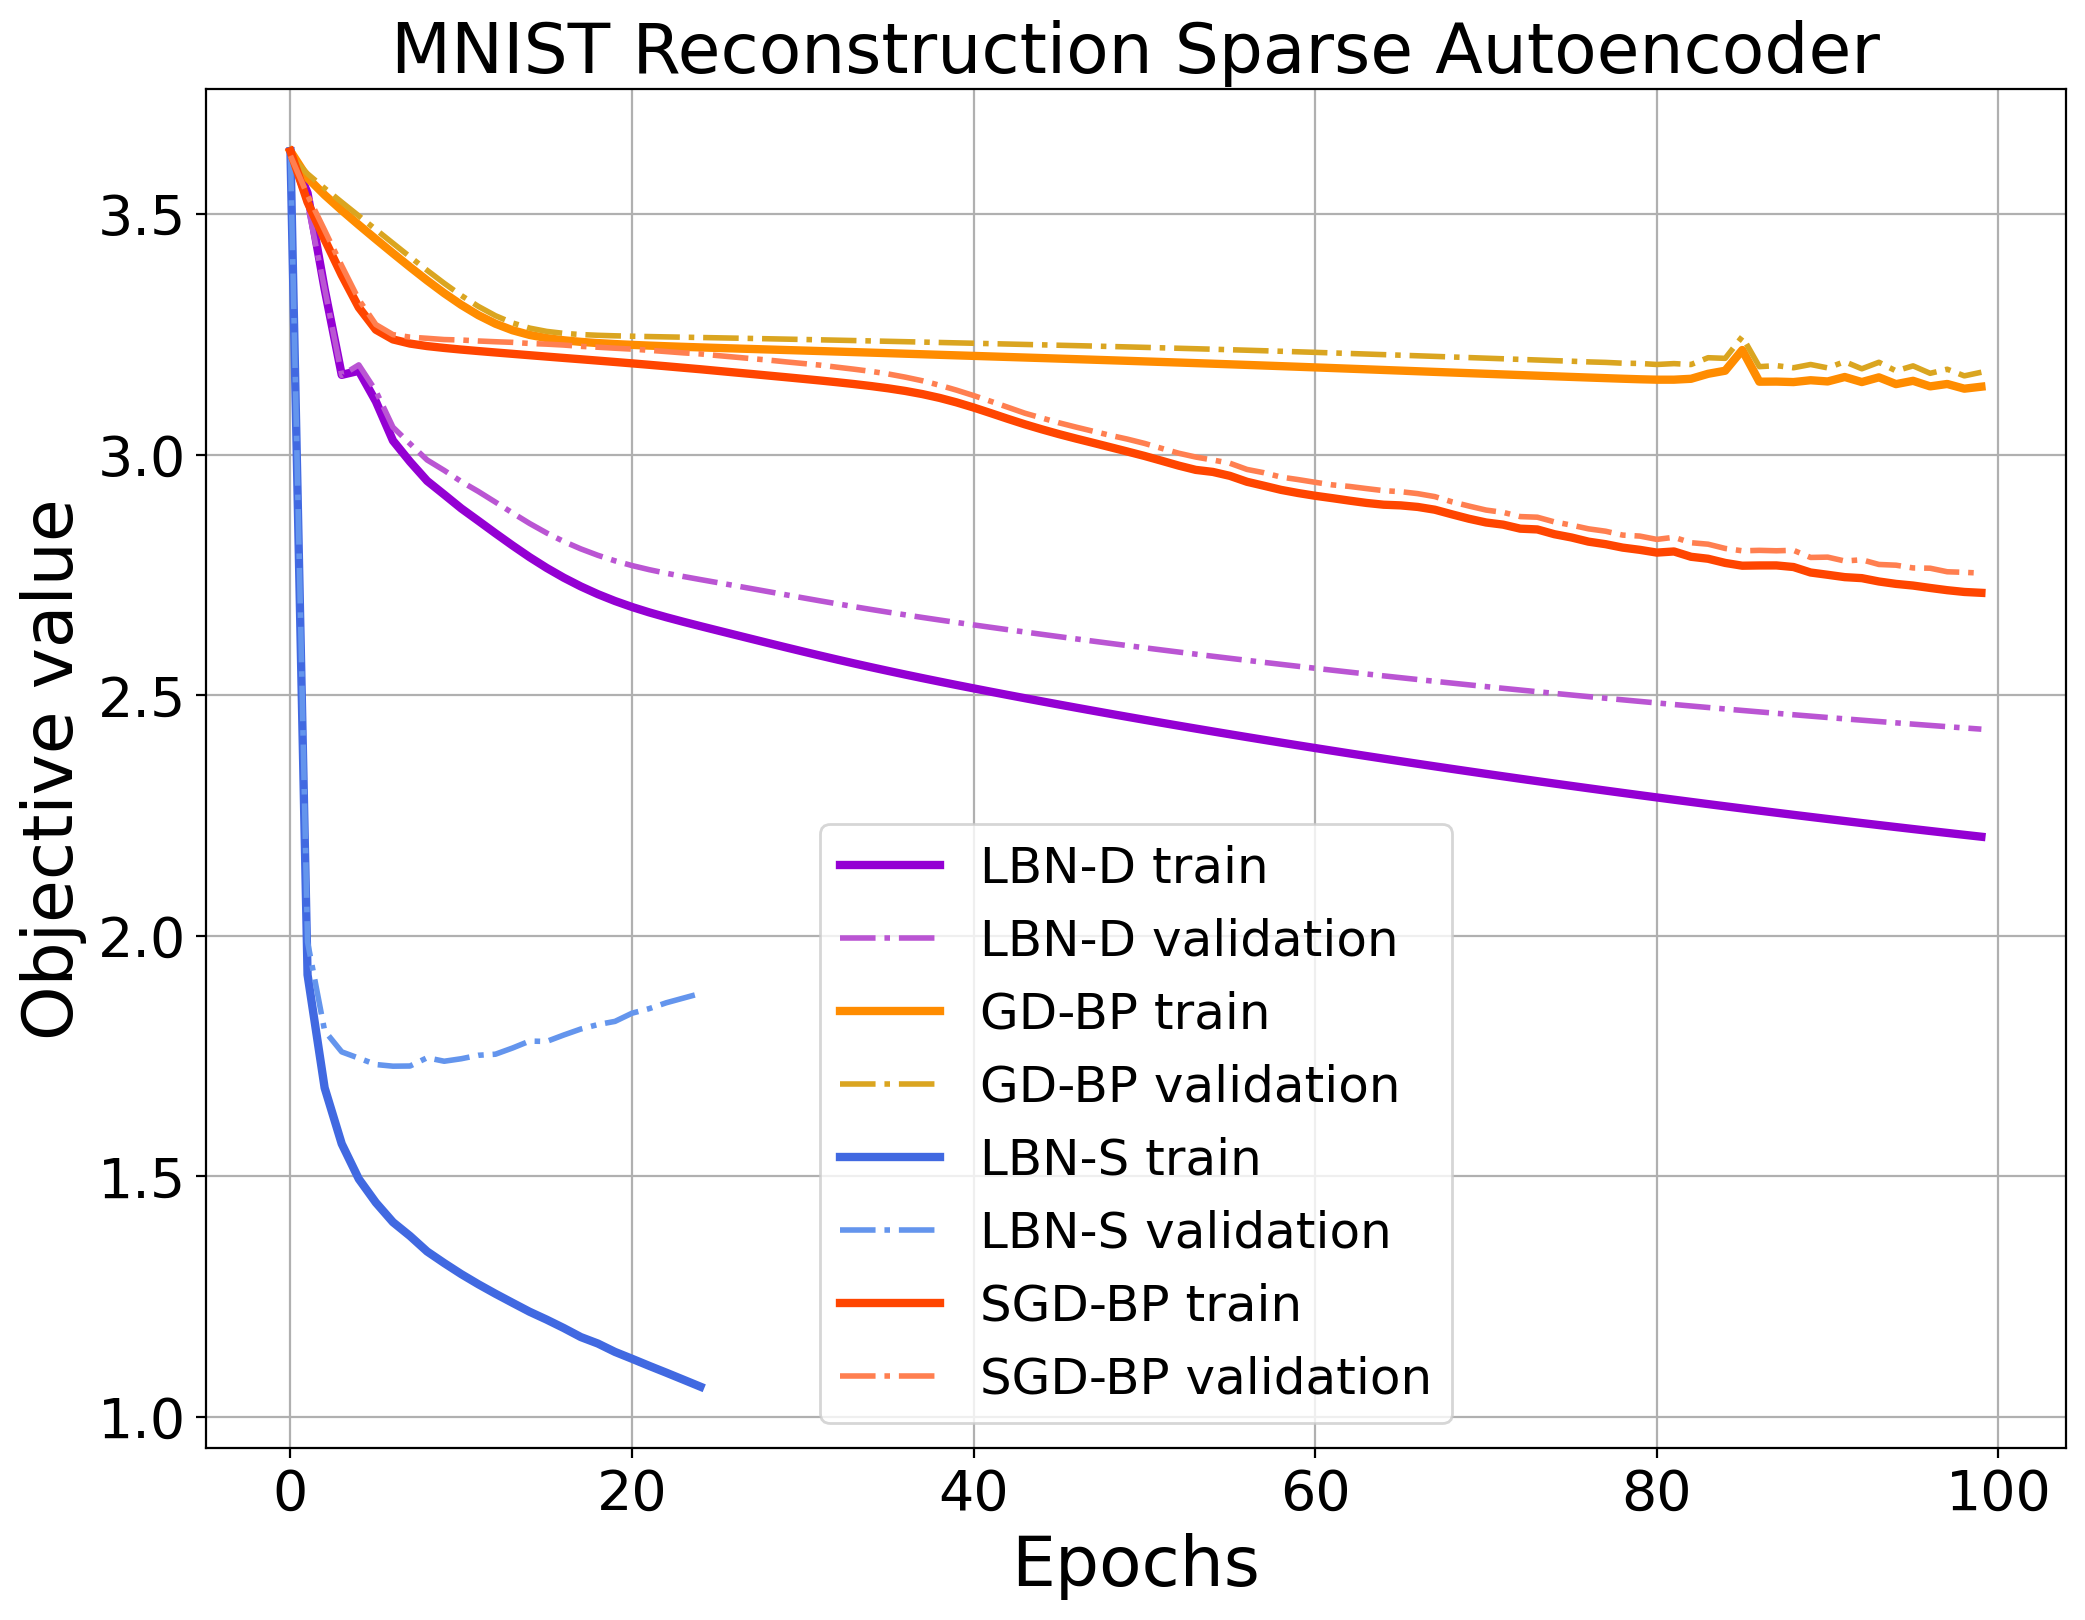
\includegraphics[width=0.48\textwidth]{../Common_Images/lifted/Numerical_Recons_SAE_MNIST_objective_all_models.png}
    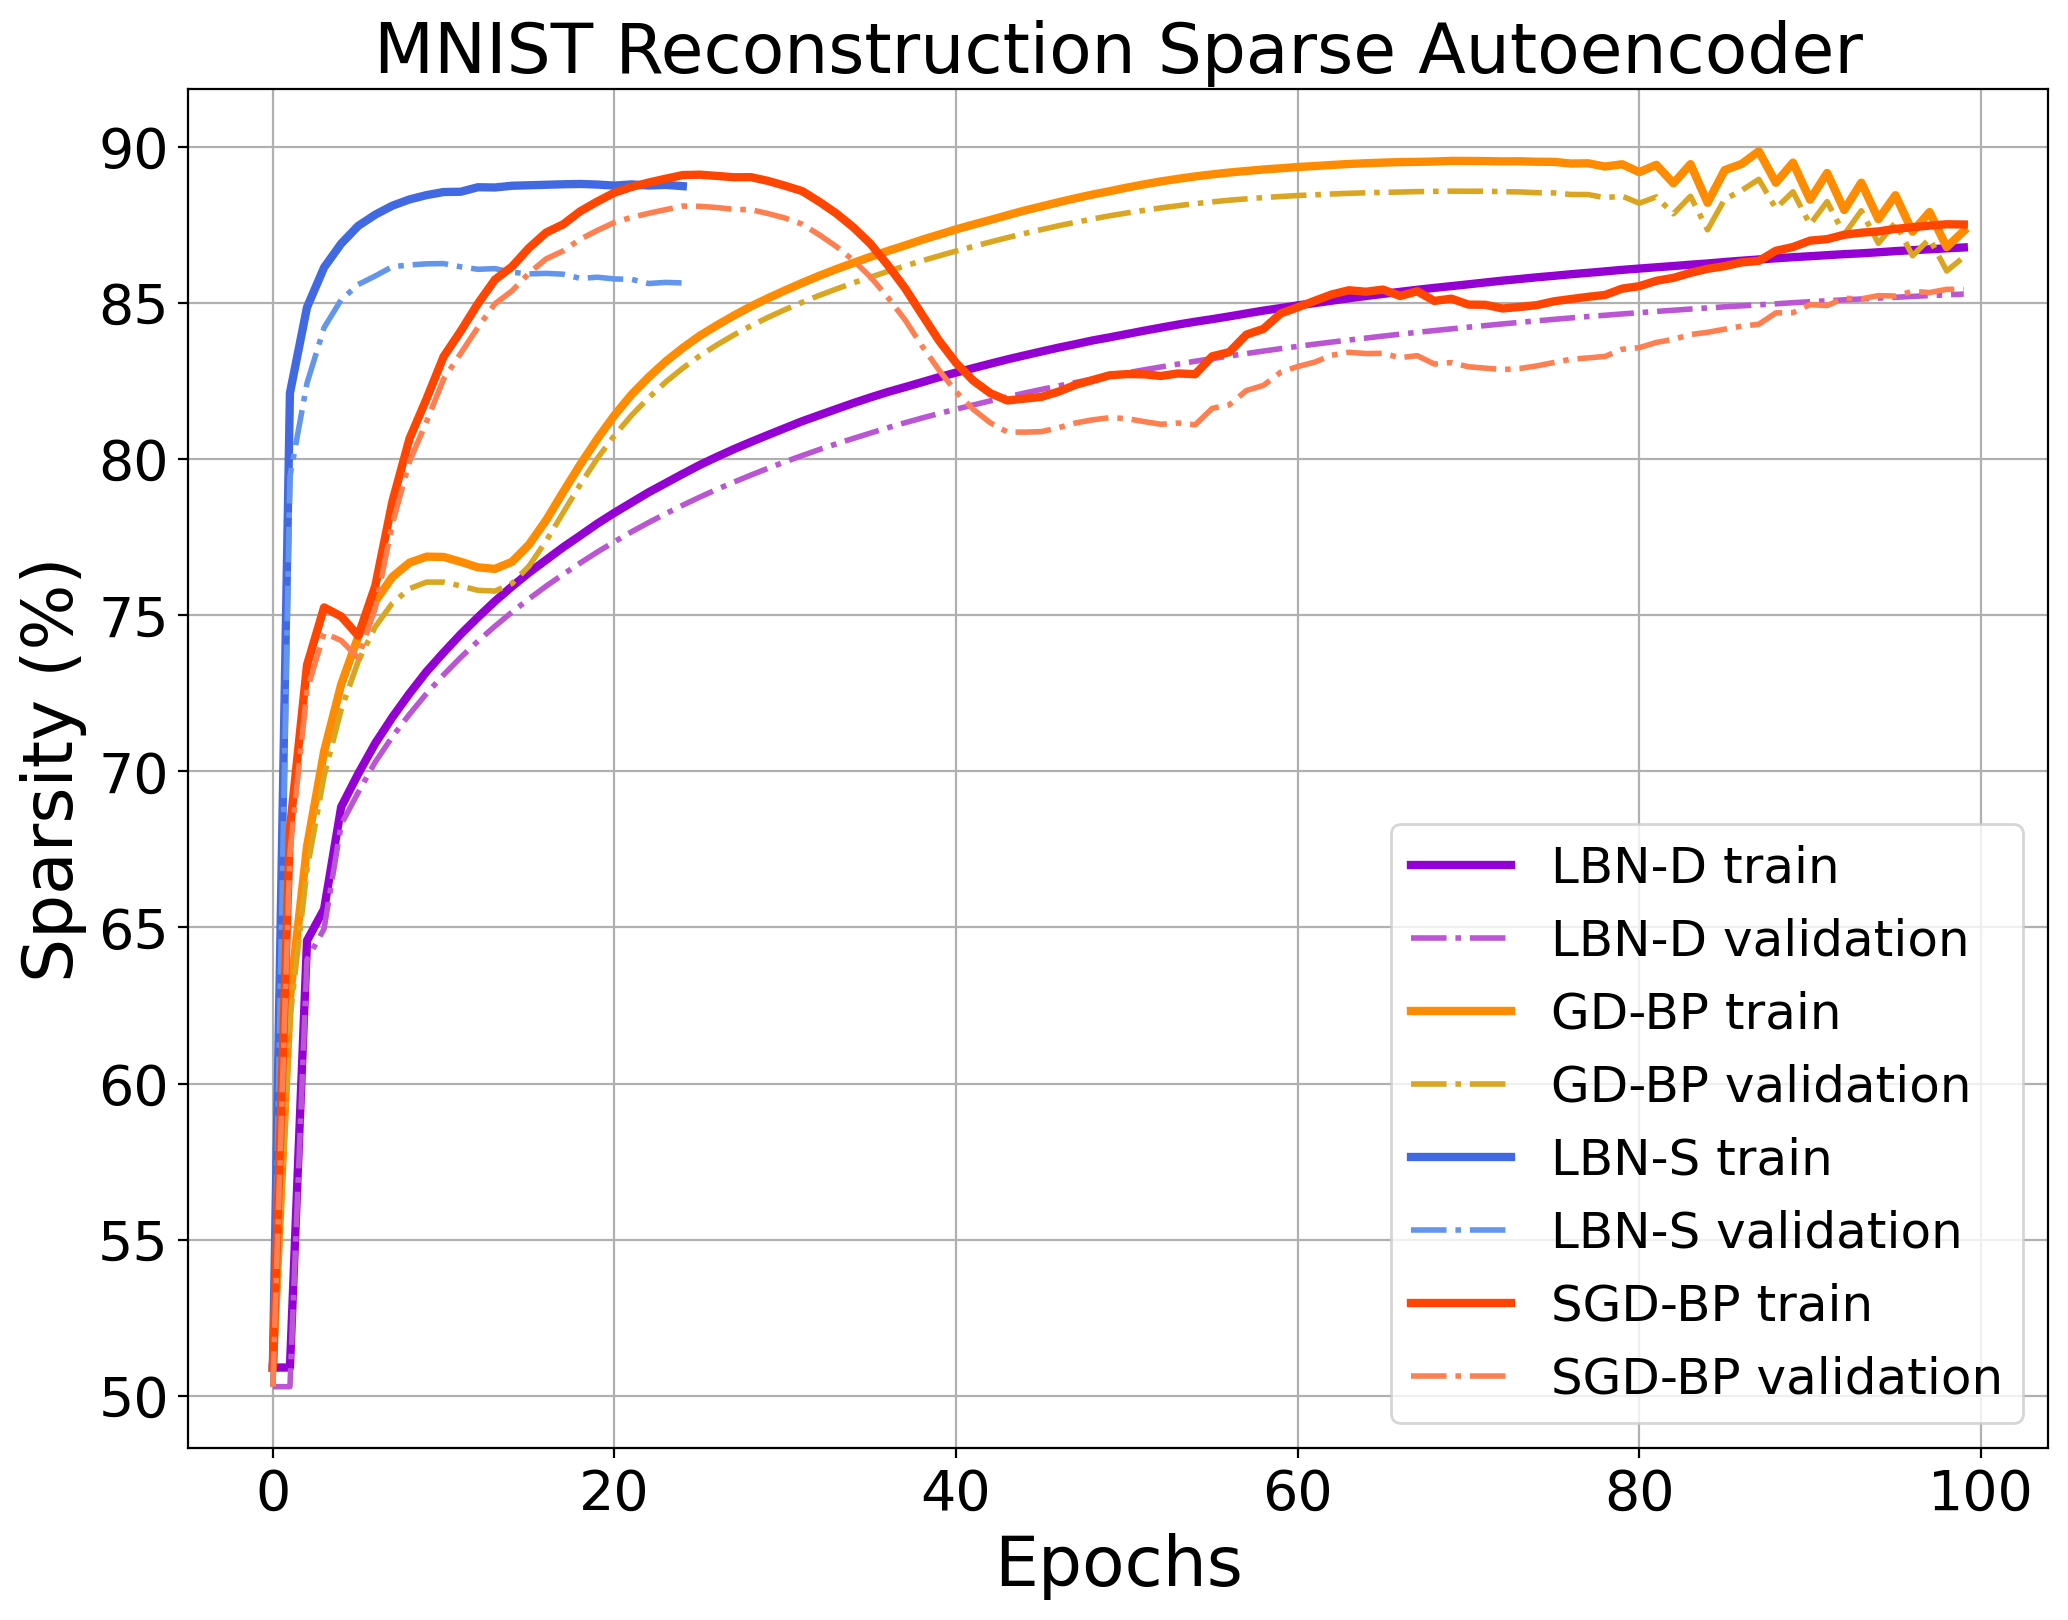
\includegraphics[width=0.48\textwidth]{../Common_Images/lifted/Numerical_Recons_SAE_MNIST_sparsity_all_models.png}
    \\
    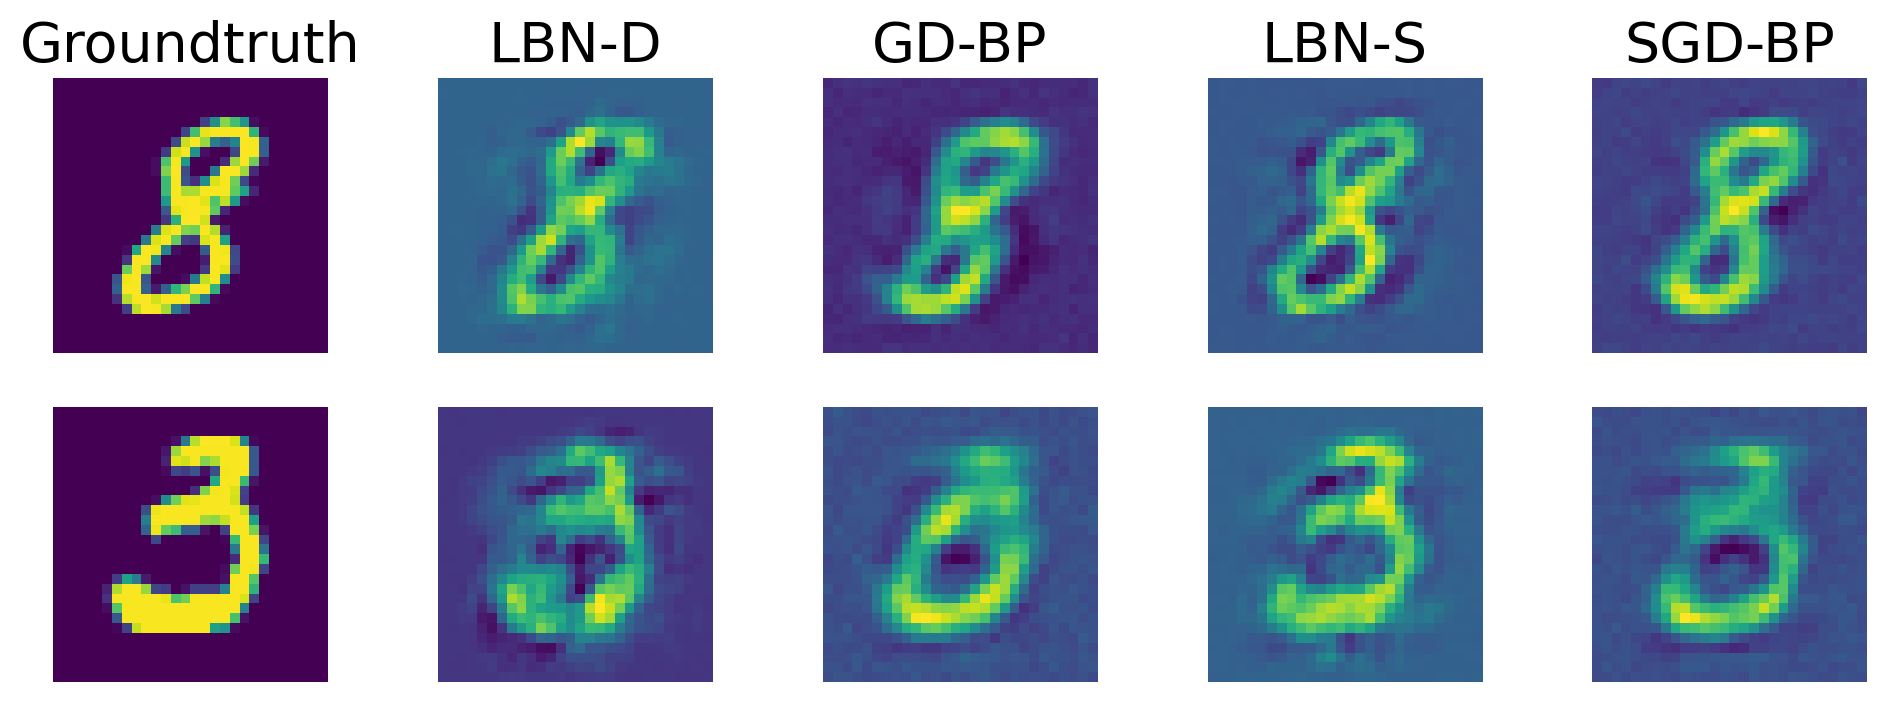
\includegraphics[width=0.85\textwidth]{../Common_Images/lifted/Numerical_Recons_SAE_MNIST_Recons_2_Val_Samples.png}
    \caption{Numerical illustration of lifted Bregman training on sparse autoencoder tasks (adapted from \cite{WangBenning2023}). Top left: training and validation objective trajectories. Top right: sparsity evolution of the latent code across epochs. Bottom: reconstruction quality on validation samples compared across optimisation strategies.}
    \label{fig:lifted_bregman_numerical_snapshot}
\end{figure}

\subsection{Generalised Perceptron Learning}
The versatility of proximal representations seamlessly encompasses seminal architectures. In Chapter~\ref{chap:nn_reg}, Section~\ref{sec:deep-learning}, we introduced the general DNN model \eqref{eq:dnn} and discussed perceptrons as the simplest instance of this architecture. We now revisit Rosenblatt's classical perceptron \cite{rosenblatt1957, rosenblatt1958} through the lifted Bregman lens. Consider a one-layer model
\begin{equation}\label{eq:perceptron_model}
    \hat y = \sigma\left(W^\top x + b\right) \, ,
\end{equation}
with weights $W$, bias $b$, input $x$, and activation $\sigma = \operatorname{prox}_{\Psi}$. In relation to the lifted objective \eqref{eq:bregman_lifted}, this is the single-block special case where one affine map $z = W^\top x + b$ is penalised against the target output via one Bregman term. Equivalently, it can be read as a one-layer reduction of the lifted philosophy from Section~\ref{sec:lifted}: decouple the nonlinearity through auxiliary variables and penalise consistency with a Bregman/Fenchel-Young gap.

\noindent For training samples $\{(x^i,y^i)\}_{i=1}^s$, we consider
\begin{equation}\label{eq:perceptron_bregman_objective}
    \min_{W,b}\; \frac{1}{s}\sum_{i=1}^s B_{\Psi}\!\left(y^i, W^\top x^i + b\right) + \alpha\,R(W,b) \, .
\end{equation}
Typical choices include $R(W,b)=\|W\|_1$ for sparsity, $R(W,b)=\frac12\|W\|_F^2$ for Tikhonov-type stabilisation, or mixed penalties such as $R(W,b)=\alpha_W\|W\|_1+\frac{\alpha_b}{2}\|b\|_2^2$ when one wishes to regularise weights and biases differently.
The key point is the gradient identity already established in \eqref{eq:bregman_loss_gradient}; therefore gradients with respect to $W$ and $b$ follow from the affine map $z = W^\top x + b$ alone -- no derivative of $\sigma$ is required. This is the crucial structural advantage over classical squared-loss training with non-smooth activations.

When $R \equiv 0$, incremental or mini-batch gradient descent on \eqref{eq:perceptron_bregman_objective} yields the following generalised Rosenblatt update.
\begin{algorithm}
\caption{Generalised Rosenblatt Update (Bregman Loss)}\label{alg:generalised_rosenblatt}
\begin{algorithmic}
\State \textbf{Input:} Initial $W^0, b^0$, step sizes $\{\tau_W^k\}, \{\tau_b^k\}$.
\For{$k = 0,1,2,\ldots$}
\State Choose mini-batch $B_k \subset \{1,\ldots,s\}$.
\State $g_W^k = \frac{1}{|B_k|}\sum_{i\in B_k} x^i\left(\sigma\!\left((W^k)^\top x^i + b^k\right) - y^i\right)^\top$
\State $g_b^k = \frac{1}{|B_k|}\sum_{i\in B_k} \left(\sigma\!\left((W^k)^\top x^i + b^k\right) - y^i\right)$
\State $W^{k+1} = W^k - \tau_W^k g_W^k$
\State $b^{k+1} = b^k - \tau_b^k g_b^k$
\EndFor
\end{algorithmic}
\end{algorithm}
For binary targets and threshold-type activations, this update recovers Rosenblatt's classical rule up to standard choices of scaling and batching. If $\Psi \equiv 0$, then $\sigma$ is the identity and one recovers the Adaline-type linear update.

If we include sparse regularisation $R(W,b)=\|W\|_1$ in \eqref{eq:perceptron_bregman_objective}, we obtain a direct Forward-Backward splitting scheme -- exactly the proximal-gradient template from Algorithm~\ref{alg:pgd}. The smooth part is the Bregman data term and the non-smooth part is the $\ell_1$ penalty, yielding an ISTA-type step (cf. Example~\ref{exm:ista}) on the weights. If one additionally imposes a non-smooth penalty on $b$, the same proximal step can be added for the bias block as well:
\begin{algorithm}
\caption{Rosenblatt-ISTA for Sparse Perceptrons}\label{alg:rosenblatt_ista_ch9}
\begin{algorithmic}
\State \textbf{Input:} Initial $W^0, b^0$, step sizes $\{\tau_W^k\}, \{\tau_b^k\}$, regularisation $\alpha>0$.
\For{$k = 0,1,2,\ldots$}
\State Choose mini-batch $B_k \subset \{1,\ldots,s\}$.
\State $g_W^k = \frac{1}{|B_k|}\sum_{i\in B_k} x^i\left(\sigma\!\left((W^k)^\top x^i + b^k\right) - y^i\right)^\top$
\State $g_b^k = \frac{1}{|B_k|}\sum_{i\in B_k} \left(\sigma\!\left((W^k)^\top x^i + b^k\right) - y^i\right)$
\State $\widetilde W^{k+1} = W^k - \tau_W^k g_W^k$
\State $W^{k+1} = \operatorname{prox}_{\tau_W^k\alpha\|\cdot\|_1}(\widetilde W^{k+1})$
\State $b^{k+1} = b^k - \tau_b^k g_b^k$
\EndFor
\end{algorithmic}
\end{algorithm}
Figure~\ref{fig:generalised_perceptron_numerical_snapshot} provides a direct numerical comparison for this sparse-perceptron setting, showing both objective decay and accuracy trajectories across optimisation strategies.

To complement Algorithms~\ref{alg:generalised_rosenblatt} and \ref{alg:rosenblatt_ista_ch9}, we include a numerical snapshot for sparse perceptron training on Fashion-MNIST from the perceptron study in \cite{wangbenning2020generalised}. The left panel tracks the regularised objective over iterations, and the right panel reports training/validation accuracy evolution.
\begin{figure}[ht]
    \centering
    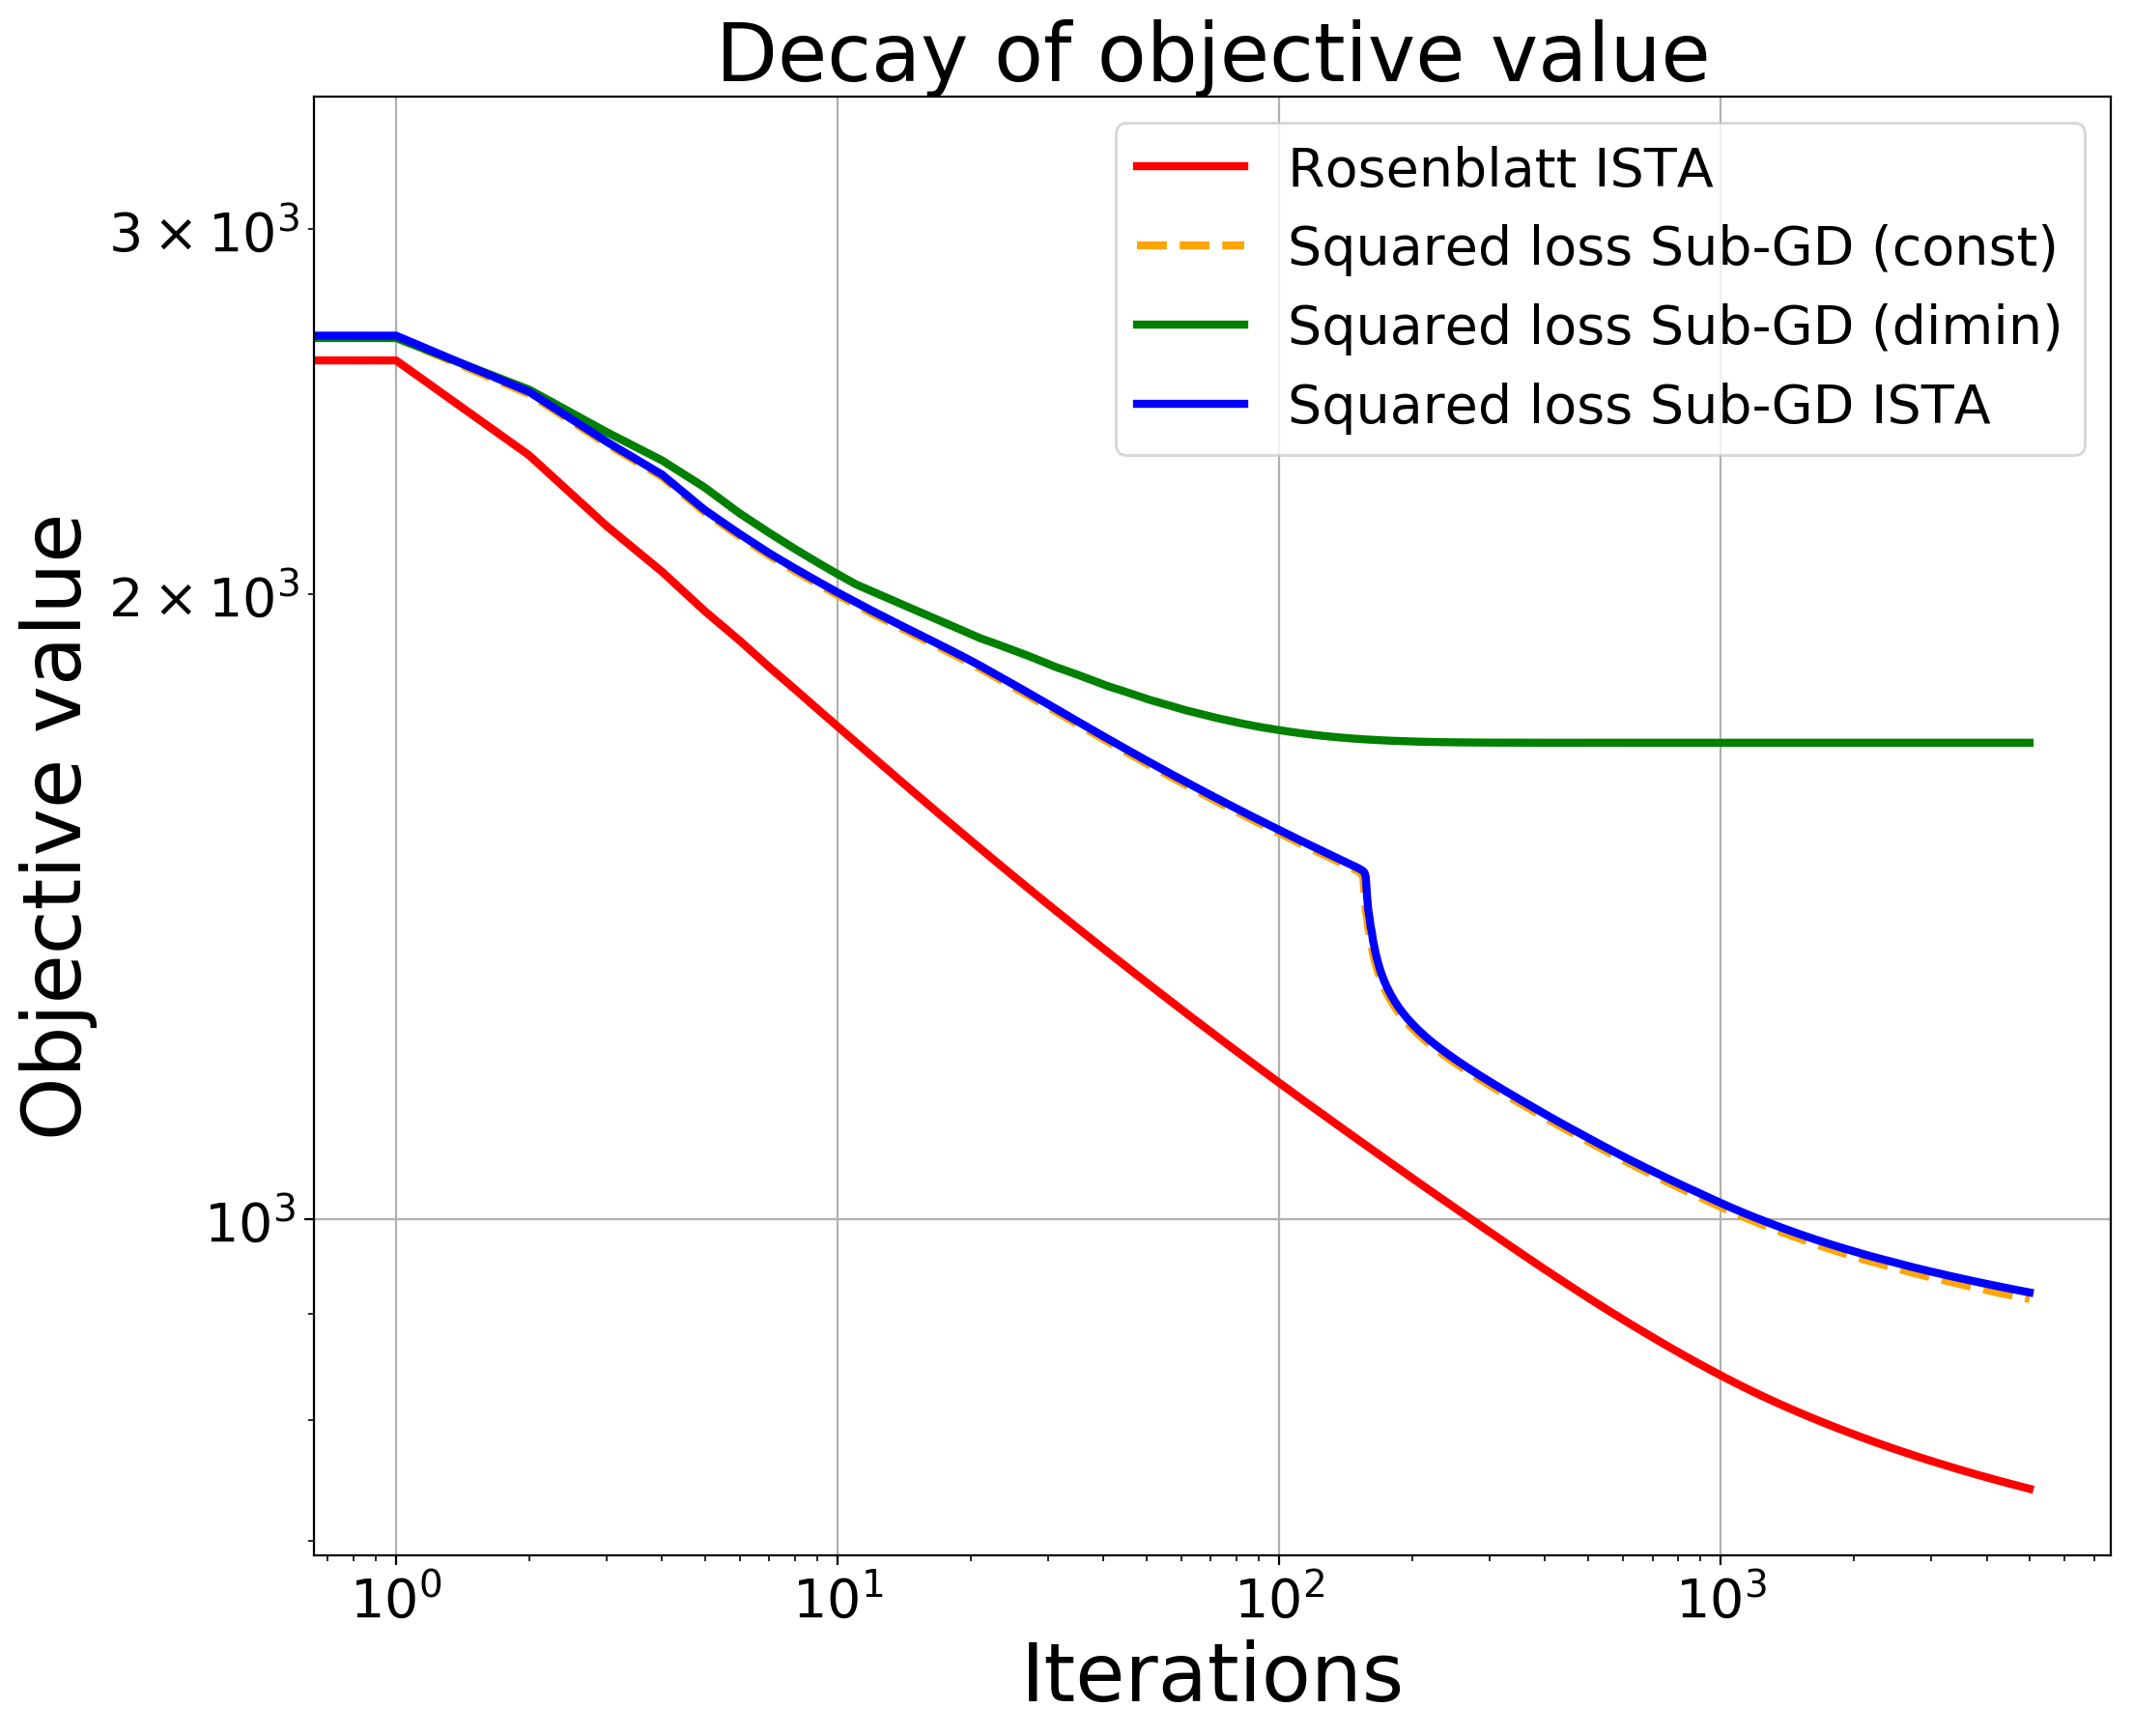
\includegraphics[width=0.48\textwidth]{../Common_Images/lifted/rosenblatt_ista_fmnist_obj_over_iterations_logx.png}
    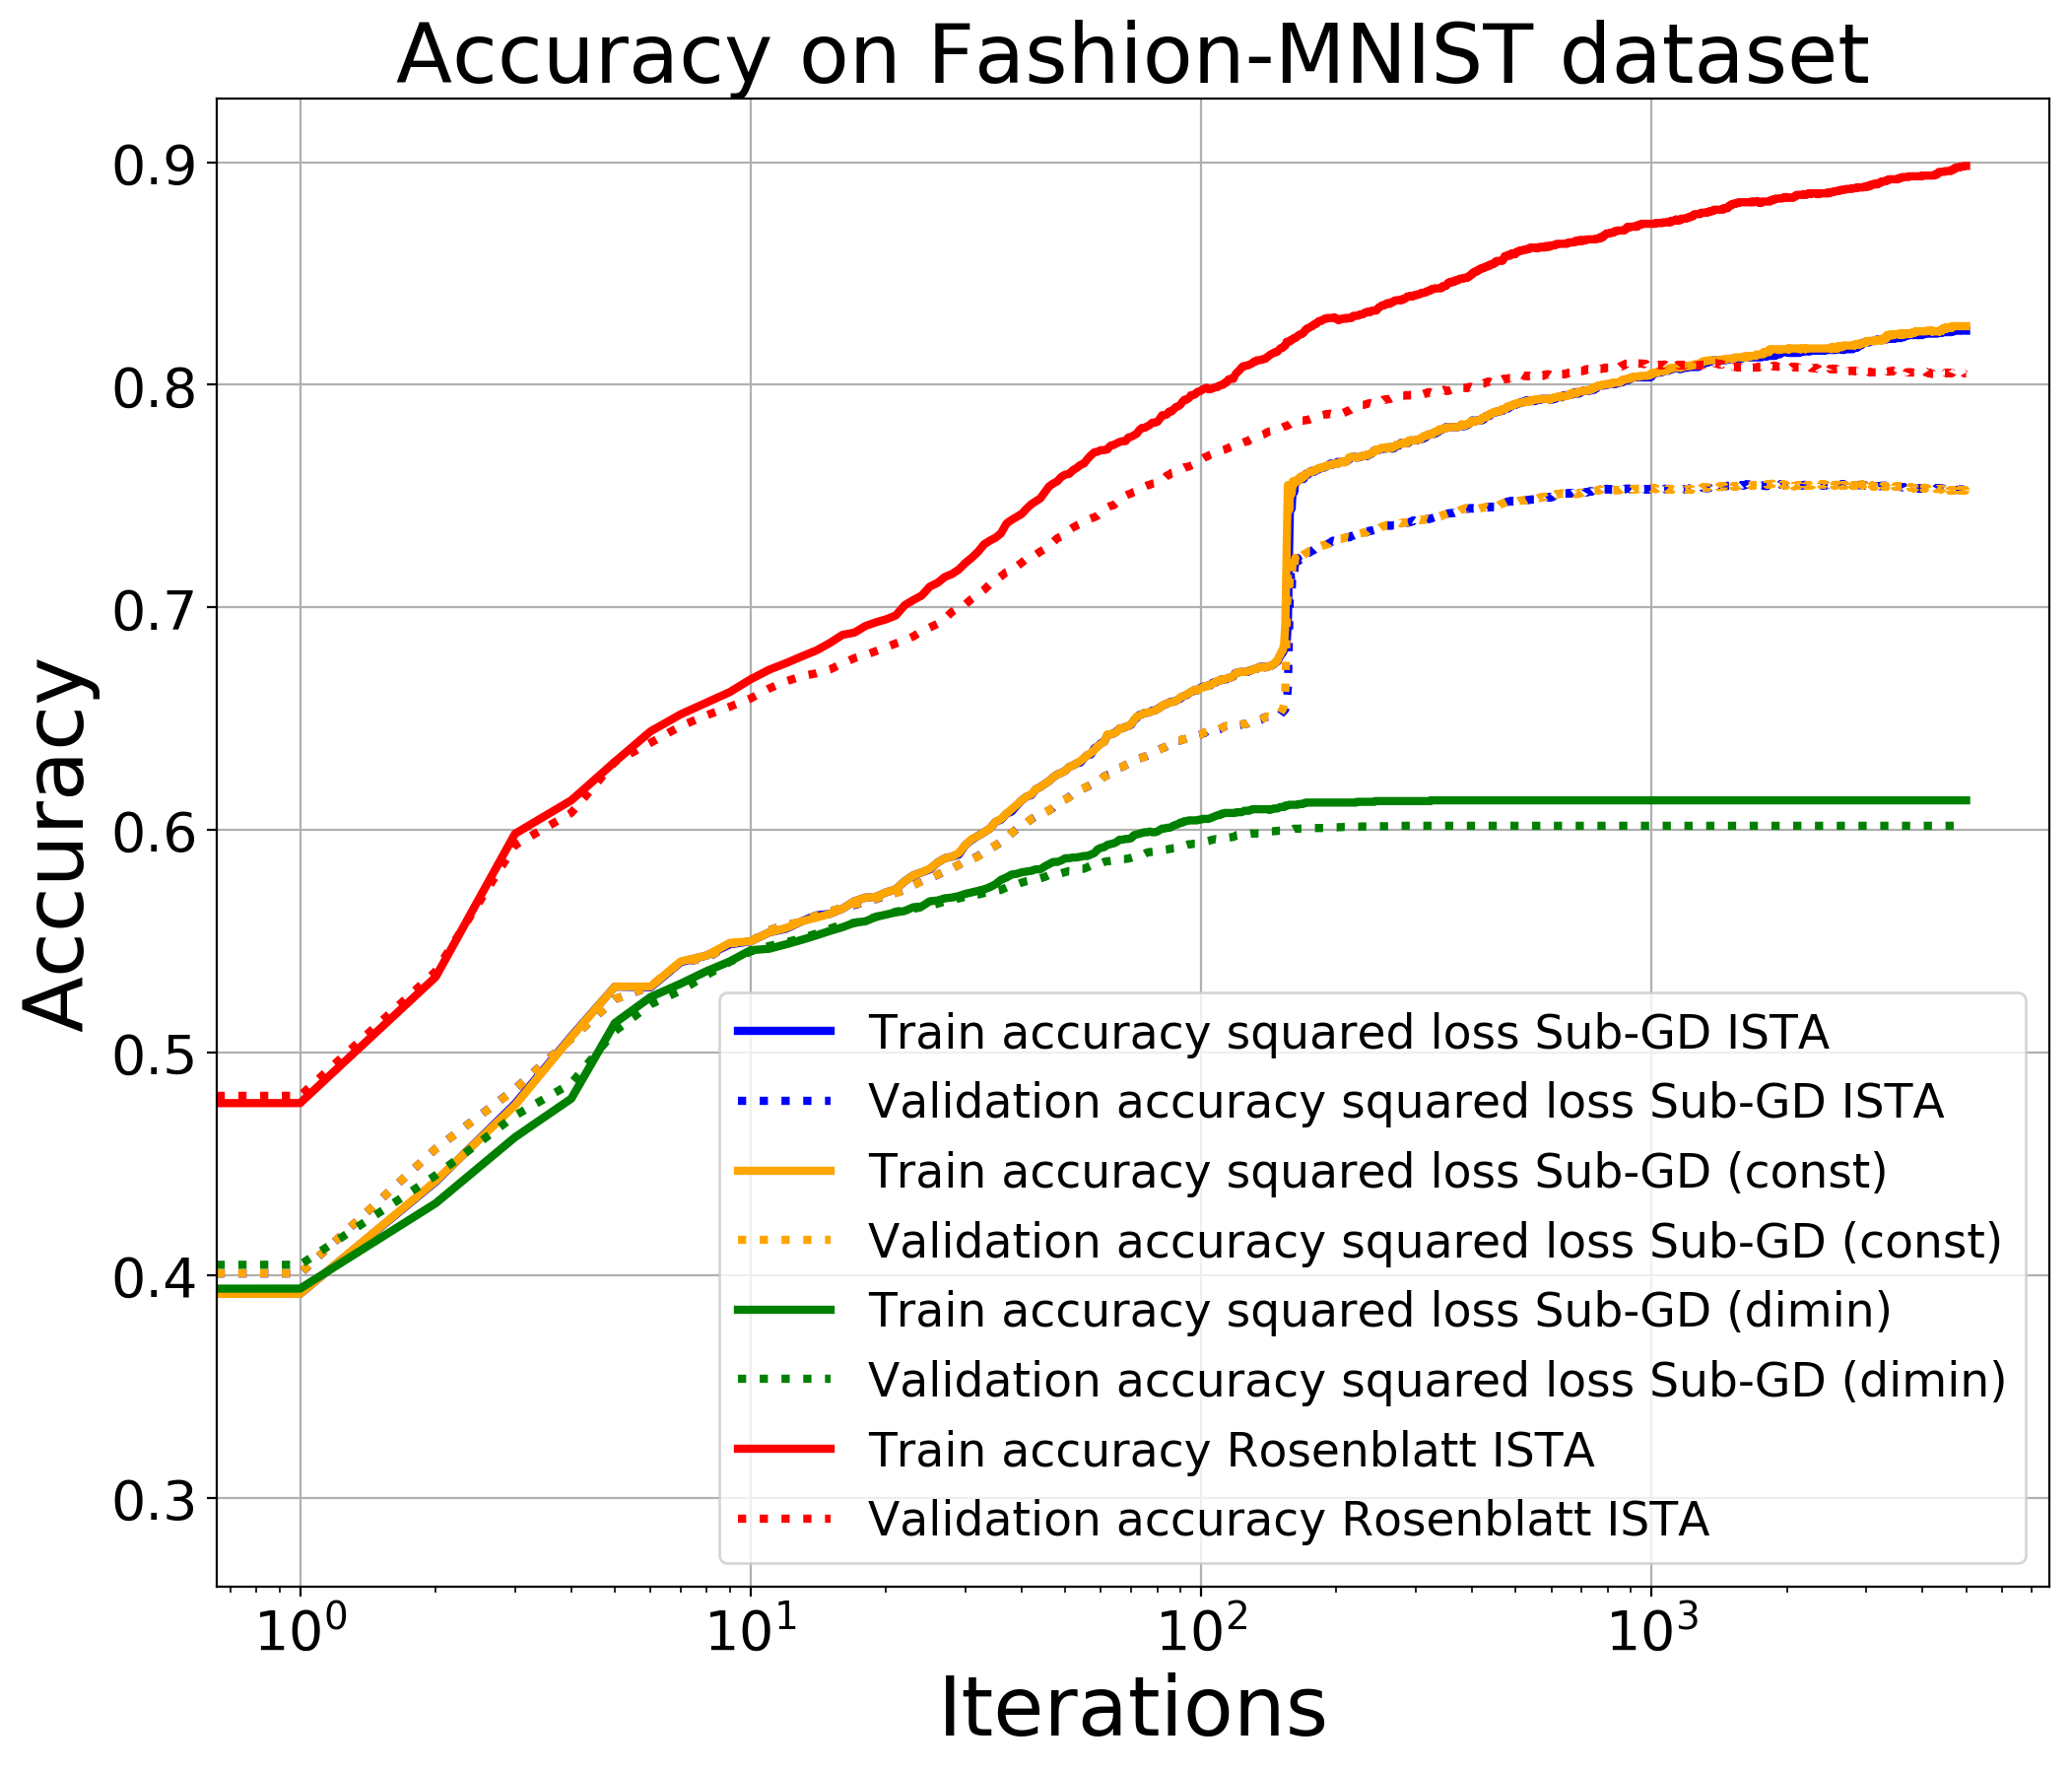
\includegraphics[width=0.48\textwidth]{../Common_Images/lifted/rosenblatt_ista_fmnist_acc_over_iterations_logx.png}
    \caption{Numerical illustration for generalised perceptron learning with sparse regularisation. Left: objective decay (Bregman-loss-based Rosenblatt-ISTA versus squared-loss baselines). Right: training and validation accuracy over iterations on Fashion-MNIST.}
    \label{fig:generalised_perceptron_numerical_snapshot}
\end{figure}
Hence, the perceptron setting provides a concrete and minimal instance of the lifted philosophy: one keeps proximal non-linearities explicit, trains without differentiating them, and directly reuses the algorithmic machinery from Chapter~\ref{ch:unrolling}.

\section{Unified Architectures and Computational Optimisation Strategies}

Having established the Bregman framework's theoretical properties, we now translate it into practice by developing a unified block-operator representation that encompasses diverse network architectures —- single-layer perceptrons, shallow networks, multi-layer MLPs, residual networks, and unrolled algorithmic networks (PNNs) —- under a single mathematical grammar. This unified perspective reveals that the distinction between conventional and lifted training is not architectural but rather a choice of penalty terms: swapping hard constraints for soft convex relaxations via Bregman distances. We then discuss the algorithmic consequences: how lifted objectives decompose into layer-wise or sample-wise subproblems that are amenable to distributed block-coordinate descent, proximal-gradient methods, and mini-batched implicit solvers. Finally, we illustrate how this framework naturally extends from training to practical applications such as sparse and denoising autoencoders, unfolded variational networks, and—most importantly—stable network inversion.

\subsection{A Unified Framework for Network Architectures}
In order to encapsulate a wide variety of neural network architectures, we can introduce a general block-operator framework. Diverse neural models can be abstractly represented via a unified system of equations. For an input vector $y$, the predicted output $N(y)$ produced by the network is determined by the output of a combined system
\begin{align}
    \label{eq:unified_architecture}
    N(y) &= A u + d \, , \\
    M u &= V z \, , \\
    z &= \sigma(W u + b) \, ,
\end{align}
where $u$ represents the structured collection of hidden or pre-activation states across all layers, $z$ denotes the corresponding post-activation variables, while $A, M, V,$ and $W$ are suitably chosen block-linear operators, and $b$ and $d$ are bias terms. The operator $A$ extracts the final readout from the stacked state $u$, the pair $(M,V)$ encodes how neighbouring blocks are coupled, and $W$ collects the affine maps to which the non-linearity $\sigma$ is applied. In this way, \eqref{eq:unified_architecture} separates three ingredients that are otherwise intertwined in the standard forward recursion: readout, linear coupling between layers, and non-linear activation.

\noindent For training samples $\{(x^i,y^i)\}_{i=1}^s$, this architecture induces the generic lifted objective
\begin{equation}\label{eq:unified_lifted_objective}
    \min_{\mathbf{\Theta},\{u^i,z^i\}_{i=1}^s} \frac{1}{s}\sum_{i=1}^s \left[ \ell\left(y^i, A u^i + d\right) + \mathcal{C}\left(Mu^i, Vz^i\right) + \mathcal{D}_{\sigma}\left(z^i, Wu^i + b\right) \right] \, ,
\end{equation}
where $\mathbf{\Theta}$ denotes the learnable entries of the block operators and biases, $\mathcal{C}$ penalises violations of the architectural coupling $Mu=Vz$, and $\mathcal{D}_{\sigma}$ penalises violations of the activation relation $z=\sigma(Wu+b)$. This is the main structural point missing from a purely architectural discussion: once \eqref{eq:unified_architecture} is written down, the difference between conventional and lifted training is encoded by the choice of these two penalty terms.

Indeed, conventional training is recovered when both constraints are enforced exactly, for example through characteristic functions,
\begin{equation}\label{eq:unified_hard_constraints}
    \mathcal{C}(a,a') = \chi_{\{0\}}(a-a') \, , \qquad \mathcal{D}_{\sigma}(z,v) = \chi_{\{0\}}\!\left(z-\sigma(v)\right) \, .
\end{equation}
Soft relaxations of \eqref{eq:unified_hard_constraints} then produce the various lifted schemes discussed earlier in this chapter: quadratic penalties recover MAC-type objectives, Fenchel-Young or biconvex penalties recover Fenchel-lifted formulations, and choosing $\mathcal{D}_{\sigma}$ as a Bregman loss yields the lifted Bregman model \eqref{eq:bregman_lifted}. Thus the unified block framework is not merely a convenient notation; it is a single template from which the main lifted training paradigms arise by changing the penalty model rather than the network architecture itself.

To make \eqref{eq:unified_architecture} concrete, we now instantiate it for the main architecture classes.

\paragraph{Single-layer perceptrons.}
To write a perceptron \eqref{eq:perceptron_model} in the form of \eqref{eq:unified_lifted_objective}, i.e.,
\begin{equation*}
    N(x) = \sigma(w^\top x + b) \, , \qquad x \in \mathbb{R}^{M} \, ,
\end{equation*}
we introduce an auxiliary scalar $\zeta$ and define $u=(x,\zeta)^\top \in \mathbb{R}^{M+1}$. Choosing
\begin{equation*}
    W = \begin{pmatrix} w^\top & 0 \end{pmatrix} \in \mathbb{R}^{1\times(M+1)} \, , \quad
    b\in\mathbb{R} \, , \quad
    M=A=\begin{pmatrix}0_{1\times M} & 1\end{pmatrix} \in \mathbb{R}^{1\times(M+1)} \, , \quad
    V=1 \, , \quad d=0 \, ,
\end{equation*}
we obtain $Mu=Vz$ as $\zeta=z$ and therefore $N(x)=Au=\zeta=\sigma(w^\top x+b)$. For vector-valued perceptrons $N(x)=\sigma(\widetilde W x+b)$ with $\widetilde W\in\mathbb{R}^{N\times M}$, we set $u=(x,\zeta)^\top\in\mathbb{R}^{M+N}$, $\zeta\in\mathbb{R}^{N}$, $W=(\widetilde W,0_{N\times N})$, $M=A=(0_{N\times M},I_N)$, and $V=I_N$.

\paragraph{Shallow neural networks.}
For the model in \eqref{eq:shallownn}, i.e.,
\begin{equation*}
    N(x)=\sum_{j=1}^{J} c_j\,\sigma_j(w_j^\top x+b_j) \, ,
\end{equation*}
we define $u=(x,h_1,\ldots,h_J)^\top\in\mathbb{R}^{M+J}$ and $z=(h_1,\ldots,h_J)^\top\in\mathbb{R}^{J}$. Then one convenient choice to frame \eqref{eq:shallownn} as \eqref{eq:unified_architecture} is with
\begin{equation*}
    A=\begin{pmatrix}0_{1\times M}&c_1&\cdots&c_J\end{pmatrix} \, , \qquad
    M=\begin{pmatrix}0_{J\times M}&I_J\end{pmatrix} \, , \qquad
    V=I_J \, ,
\end{equation*}
and
\begin{equation*}
    W=
    \begin{pmatrix}
        w_1^\top & 0 & \cdots & 0\\
        w_2^\top & 0 & \cdots & 0\\
        \vdots & \vdots & \ddots & \vdots\\
        w_J^\top & 0 & \cdots & 0
    \end{pmatrix}
    \in \mathbb{R}^{J\times(M+J)} \, ,
\end{equation*}
with activation acting component-wise, i.e. $\sigma=(\sigma_1,\ldots,\sigma_J)^\top$.

\paragraph{Multi-layer perceptrons.}
For an $L$-layer MLP with weight matrices $W_l \in \mathbb{R}^{N_l \times N_{l-1}}$ (where $N_0 = M$ is the input dimension and $N_l$ is the width of the $l$-th hidden layer), bias vectors $b_l \in \mathbb{R}^{N_l}$, and output weight $K \in \mathbb{R}^{N \times N_L}$, the forward pass reads
\begin{equation*}
    x^l = \sigma_l(W_l x^{l-1} + b_l) \quad (l=1,\ldots,L) \, , \qquad x^0 = x \, , \qquad N(x) = Kx^L + d \, .
\end{equation*}
Define the stacked variable $u = \bigl((x^0)^\top, (x^1)^\top, \ldots, (x^L)^\top\bigr)^\top \in \mathbb{R}^{\bar{N}}$, where $\bar{N} = \sum_{l=0}^L N_l$, and $z = \bigl((z^1)^\top, \ldots, (z^L)^\top\bigr)^\top \in \mathbb{R}^{\bar{N}-N_0}$ with $z^l = x^l$. The operators in \eqref{eq:unified_architecture} then take the explicit form \cite{wang2025unified}
\begin{align*}
    W = \begin{pmatrix}
        W_1 & 0_{N_1 \times N_1} & 0_{N_1 \times N_2} & \cdots & 0_{N_1 \times N_{L-1}} & 0_{N_1 \times N_L} \\
        0_{N_2 \times N_0} & W_2 & 0_{N_2 \times N_2} & \cdots & 0_{N_2 \times N_{L-1}} & 0_{N_2 \times N_L} \\
        \vdots & & \ddots & & \vdots & \vdots \\
        0_{N_L \times N_0} & \cdots & & & W_L & 0_{N_L \times N_L}
    \end{pmatrix} \in \mathbb{R}^{(\bar{N}-N_0) \times \bar{N}} \, ,
\end{align*}
with bias $b = (b_1, \ldots, b_L)^\top \in \mathbb{R}^{\bar{N}-N_0}$,
\begin{align*}
    M = \begin{pmatrix}
        0_{N_1 \times N_0} & I_{N_1} & 0_{N_1 \times N_2} & 0_{N_1 \times N_3} & \cdots & 0_{N_1 \times N_L} \\
        0_{N_2 \times N_0} & 0_{N_2 \times N_1} & I_{N_2} & 0_{N_2 \times N_3} & \cdots & 0_{N_2 \times N_L} \\
        \vdots & \vdots & & \ddots & & \vdots \\
        0_{N_L \times N_0} & 0_{N_L \times N_1} & \cdots & & & I_{N_L}
    \end{pmatrix} \in \mathbb{R}^{(\bar{N}-N_0) \times \bar{N}} \, ,
\end{align*}
$V = I_{\bar{N}-N_0}$, and
\begin{equation*}
    A = \begin{pmatrix} 0_{N \times N_0} & 0_{N \times N_1} & \cdots & 0_{N \times N_{L-1}} & K \end{pmatrix} \in \mathbb{R}^{N \times \bar{N}} \, .
\end{equation*}
The matrix $W$ is block sub-diagonal: in row $l$, the block $W_l$ occupies the block-column corresponding to $x^{l-1}$ and all remaining entries are zero, so $Wu + b$ assembles the pre-activations $(W_1 x^0 + b_1, \ldots, W_L x^{L-1} + b_L)^\top$. The matrix $M$ is a block identity shift extracting the post-activation states $(x^1, \ldots, x^L)$ from $u$; since $V = I$, the constraint $Mu = Vz$ simply asserts $z^l = x^l$. The output map $A$ zeros all but the final block $x^L$ and applies $K$ to produce $Kx^L + d$. The activation vector $\sigma = (\sigma_1, \ldots, \sigma_L)^\top$ acts independently on each pre-activation, completing the feed-forward encoding.

\paragraph{Residual networks.}
For an $L$-block ResNet \cite{He2016resnet} with all layers sharing the same channel width $M$, weight matrices $W_l \in \mathbb{R}^{N_l \times M}$ and $V_l \in \mathbb{R}^{M \times N_l}$, scalar step-sizes $h_l > 0$, and output weight $K \in \mathbb{R}^{N \times M}$, the residual update and network output read
\begin{equation*}
    x^l = x^{l-1} + h_l V_l \sigma_l(W_l x^{l-1} + b_l) \quad (l=1,\ldots,L) \, , \qquad N(x) = Kx^L + d \, .
\end{equation*}
We define $u = \bigl((x^0)^\top, (x^1)^\top, \ldots, (x^L)^\top\bigr)^\top \in \mathbb{R}^{M(L+1)}$ and $z = \bigl((z^1)^\top, \ldots, (z^L)^\top\bigr)^\top \in \mathbb{R}^{\bar{N}}$ with $\bar{N} = \sum_{l=1}^L N_l$. The operators in \eqref{eq:unified_architecture} are \cite{wang2025unified}
\begin{align*}
    W = \begin{pmatrix}
        W_1 & 0_{N_1 \times M} & 0_{N_1 \times M} & \cdots & 0_{N_1 \times M} & 0_{N_1 \times M} \\
        0_{N_2 \times M} & W_2 & 0_{N_2 \times M} & \cdots & 0_{N_2 \times M} & 0_{N_2 \times M} \\
        \vdots & & \ddots & & \vdots & \vdots \\
        0_{N_L \times M} & \cdots & & & W_L & 0_{N_L \times M}
    \end{pmatrix} \in \mathbb{R}^{\bar{N} \times M(L+1)} \, ,
\end{align*}
with bias $b = (b_1, \ldots, b_L)^\top \in \mathbb{R}^{\bar{N}}$,
\begin{align*}
    M = \begin{pmatrix}
        -I_M & I_M & 0_M & 0_M & \cdots & 0_M \\
        0_M & -I_M & I_M & 0_M & \cdots & 0_M \\
        \vdots & \vdots & & \ddots & \ddots & \vdots \\
        0_M & 0_M & \cdots & & -I_M & I_M
    \end{pmatrix} \in \mathbb{R}^{ML \times M(L+1)} \, ,
\end{align*}
\begin{align*}
    V = \begin{pmatrix}
        h_1 V_1 & 0_{M \times N_2} & \cdots & 0_{M \times N_L} \\
        0_{M \times N_1} & h_2 V_2 & \cdots & 0_{M \times N_L} \\
        \vdots & & \ddots & \vdots \\
        0_{M \times N_1} & \cdots & & h_L V_L
    \end{pmatrix} \in \mathbb{R}^{ML \times \bar{N}} \, ,
\end{align*}
and
\begin{equation*}
    A = \begin{pmatrix} 0_{N \times M} & 0_{N \times M} & \cdots & 0_{N \times M} & K \end{pmatrix} \in \mathbb{R}^{N \times M(L+1)} \, .
\end{equation*}
The matrix $M$ is a block first-difference operator: row $l$ computes $x^l - x^{l-1}$. The matrix $V$ is block-diagonal with the scaled residual weights $h_l V_l$ on its diagonal blocks, adjusting the width and magnitude of each shortcut. The coupling constraint $Mu = Vz$ therefore reads $x^l - x^{l-1} = h_l V_l z^l$ for each $l$, which combined with the activation relation $z^l = \sigma_l(W_l x^{l-1} + b_l)$ recovers the residual update. The output map $A$ selects the final state $x^L$ and applies $K$. The analogy to forward Euler discretisation of an ODE is transparent from the form of $M$ and $V$ (cf.\ Chapter~\ref{ch:continuous_dynamics}); different time-integration schemes correspond directly to different designs of these two operators \cite{benning2019deep}.

\paragraph{Proximal neural networks and LISTA-type unrolling.}
The Learned Iterative Soft-Thresholding Algorithm (LISTA, Section~\ref{sec:lista}) constructs a neural network by unrolling $J$ steps of the ISTA algorithm (cf.\ Example~\ref{exm:ista}) for the sparse reconstruction problem
\begin{equation*}
    \min_{\alpha \in \mathbb{R}^P} \tfrac{1}{2}\|H\Phi\alpha - y\|_2^2 + \lambda\|\alpha\|_1 \, ,
\end{equation*}
where $\Phi \in \mathbb{R}^{N \times P}$ is a dictionary, $H \in \mathbb{R}^{M \times N}$ is the measurement operator, and $\lambda > 0$ is a regularisation parameter. With learnable step-sizes $\gamma_j > 0$, thresholds $\lambda_j > 0$, and dictionaries $\Phi_j$, the iteration reads
\begin{equation*}
    \alpha_j = \mathcal{S}_{\gamma_j\lambda_j}\!\bigl(\widetilde{W}_j\,\alpha_{j-1} + \tilde{b}_j\bigr) \quad (j=2,\ldots,J{-}1) \, ,
\end{equation*}
where $\widetilde{W}_j = I_P - \gamma_j \Phi_j^\top H^\top H \Phi_j$, $\tilde{b}_j = \gamma_j \Phi_j^\top H^\top y$, and $\mathcal{S}_\mu(z) = \operatorname{sign}(z)\max(|z|-\mu,0)$ is the soft-thresholding operator, i.e.\ $\mathcal{S}_\mu = \operatorname{prox}_{\mu\|\cdot\|_1}$. The network is initialised with $\alpha_1 = \Phi_1^\top H^\top y$ (a linear step, no thresholding) and produces output $N(y) = \Phi_J \alpha_{J-1}$. Define the stacked variable $u = (y, \alpha_1, \ldots, \alpha_{J-1})^\top \in \mathbb{R}^{M+(J-1)P}$ and $z = (\alpha_1, \ldots, \alpha_{J-1})^\top \in \mathbb{R}^{(J-1)P}$. The operators in \eqref{eq:unified_architecture} then read \cite{wang2025unified}
\begin{align*}
    W = \begin{pmatrix}
        \Phi_1^\top H^\top & 0_{P \times P} & 0_{P \times P} & \cdots & 0_{P \times P} & 0_{P \times P} \\
        0_{P \times M} & \widetilde{W}_2 & 0_{P \times P} & \cdots & 0_{P \times P} & 0_{P \times P} \\
        \vdots & & \ddots & & \vdots & \vdots \\
        0_{P \times M} & \cdots & & & \widetilde{W}_{J-1} & 0_{P \times P}
    \end{pmatrix} \in \mathbb{R}^{(J-1)P \times (M+(J-1)P)} \, ,
\end{align*}
with bias $b = (0_P, \tilde{b}_2, \ldots, \tilde{b}_{J-1})^\top \in \mathbb{R}^{(J-1)P}$ where $\tilde{b}_j = \gamma_j \Phi_j^\top H^\top y$,
\begin{align*}
    M = \begin{pmatrix}
        0_{P \times M} & I_P & 0_{P \times P} & \cdots & 0_{P \times P} \\
        0_{P \times M} & 0_{P \times P} & I_P & \cdots & 0_{P \times P} \\
        \vdots & \vdots & & \ddots & \vdots \\
        0_{P \times M} & 0_{P \times P} & \cdots & & I_P
    \end{pmatrix} \in \mathbb{R}^{(J-1)P \times (M+(J-1)P)} \, ,
\end{align*}
$V = I_{(J-1)P}$, and
\begin{equation*}
    A = \begin{pmatrix} 0_{N \times M} & 0_{N \times P} & \cdots & 0_{N \times P} & \Phi_J \end{pmatrix} \in \mathbb{R}^{N \times (M+(J-1)P)} \, .
\end{equation*}
The first row of $W$ maps the observation $y$ (the first block of $u$) through $\Phi_1^\top H^\top$ to compute the initialisation $\alpha_1$; subsequent rows apply the ISTA weight $\widetilde{W}_j$ to the preceding iterate $\alpha_{j-1}$ (the $(j-1)$-th block of $u$). The bias term $\tilde{b}_j = \gamma_j \Phi_j^\top H^\top y$ provides the data-driven forcing at each step. The matrix $M$ selects the iterate blocks $\alpha_1, \ldots, \alpha_{J-1}$ from $u$; with $V = I$ the coupling constraint $Mu = Vz$ simply asserts $z^j = \alpha_j$. The output map $A$ applies the final dictionary $\Phi_J$ to $\alpha_{J-1}$ to synthesise the signal estimate. The activation vector is $\sigma = \bigl(\operatorname{Id}, \mathcal{S}_{\gamma_2\lambda_2}, \ldots, \mathcal{S}_{\gamma_{J-1}\lambda_{J-1}}\bigr)^\top$: the first component is the identity (no thresholding on the initialisation step) and each subsequent component is a soft-thresholding operator, which is exactly $\operatorname{prox}_{\gamma_j\lambda_j\|\cdot\|_1}$. This is the key reason PNNs are central to the lifted Bregman setting: the soft-thresholding activation satisfies the proximal structure \eqref{eq:proximal_activation} by construction, so the Bregman loss \eqref{eq:bregman_loss} applies directly to every iterate update. The same viewpoint extends to learned primal-dual unrollings (Section~\ref{sec:lista}), where one stacks primal iterates $x_j$ and dual iterates $\alpha_j$ into $u$ and treats both the primal and dual proximal maps as components of $\sigma$ \cite{wang2025unified}.

\subsection{Optimisation Algorithms for Lifted Training}
To solve \eqref{eq:unified_lifted_objective} in practice, one exploits the fact that lifting trades a deeply nested dependency structure for a larger but block-separable optimisation problem. Writing the total objective as $\mathcal{J}(\mathbf{\Theta},\mathbf{X})$, where $\mathbf{X}$ collects all auxiliary variables $\{u^i,z^i\}_{i=1}^s$, a basic deterministic Block-Coordinate Descent (BCD) strategy alternates between
\begin{equation}\label{eq:unified_bcd_updates}
    \mathbf{\Theta}^{k+1} \in \argmin_{\mathbf{\Theta}} \mathcal{J}(\mathbf{\Theta},\mathbf{X}^k) \, , \qquad
    \mathbf{X}^{k+1} \in \argmin_{\mathbf{X}} \mathcal{J}(\mathbf{\Theta}^{k+1},\mathbf{X}) \, .
\end{equation}
For the lifted models discussed above, these two global blocks can be further decomposed into layer-wise or sample-wise subproblems. In particular, for MAC-, Fenchel-, and Bregman-type relaxations, the subproblems are often convex in each block even though the full objective remains non-convex. This is the mathematical reason why lifted methods are naturally compatible with distributed or parallel updates.

Exact minimisation in \eqref{eq:unified_bcd_updates} is often too expensive, so one typically uses inexact block updates based on the optimisation tools introduced earlier in the notes. In particular, proximal gradient descent (Algorithm~\ref{alg:pgd}) and ISTA-type updates (Example~\ref{exm:ista}) can be applied to parameter blocks and auxiliary-variable blocks whenever a smooth data-fit term is coupled with non-smooth regularisation.

For large datasets, these updates are naturally combined with mini-batching. Rather than solving the full lifted objective at every iteration, one works on the currently sampled batch and performs a small number of inner block updates. A particularly useful instance is the Implicit Stochastic Gradient Method (ISGM): at each stochastic step, one solves a proximal regularised local subproblem for the active batch, and this inner subproblem is approximated by the same BCD/proximal-gradient machinery just described.

Compared with explicit SGD updates, this implicit variant is often less sensitive to learning-rate choices and only requires storing auxiliary variables for the active batch. In practice, one therefore obtains a flexible hierarchy of solvers: deterministic BCD on the full objective, mini-batch BCD/proximal-gradient updates, and implicit stochastic outer iterations with proximal inner solves.

Finally, acceleration and adaptivity are natural refinements of this framework: Nesterov or Heavyball momentum can be added to gradient-type block updates, while Adam-style preconditioning can be used on parameter and/or auxiliary blocks. Consequently, lifted training is best viewed as a structured optimisation framework in which multiple algorithms from earlier chapters can be combined, rather than as one fixed update rule.

\subsection{Practical Training Applications}
In practice, the lifted formulation is most useful when one wants to regularise hidden variables directly, for example in sparse or denoising autoencoders and in unfolded proximal architectures. Since auxiliary states are explicit optimisation variables, structure-inducing penalties can be imposed and updated locally through proximal/block-wise steps, while the same block-operator model \eqref{eq:unified_architecture} is retained. This gives a natural conceptual bridge to inversion: the optimisation machinery developed for training can be reused to recover stable inputs or latent states from noisy outputs within the same lifted Bregman framework (cf.\ \cite{wang2025unified}).

\section{Regularised Inversion of Deep Neural Networks}
The lifted perspective is not only useful for \emph{training}; it also provides a principled route to \emph{inversion}. In the language of Chapter~\ref{ch:reg}, this is a variational regularisation problem of the form \eqref{eq:var_reg}, where we replace classical data terms by lifted Bregman penalties that are naturally matched to proximal activations. This yields a stable, model-based alternative to direct decoder inversion and links the optimisation machinery of this chapter to the regularisation framework developed earlier.

\subsection{Introduction to Inverse Problems}
In the preceding sections, we explored the estimation of network parameters from given training data. In contrast, we now consider the inverse problem of recovering an input or representation $u$ for a fixed, pre-trained neural network.
Suppose we are given an $L$-layer feed-forward neural network or multi-layer perceptron taking the form of \eqref{eq:dnn} for pre-trained parameters $w$. The fundamental challenge of inverse problems here is to determine internal properties of a system from indirect, noisy measurements. For given noisy data $f^\delta$, we aim to solve the nonlinear inverse problem
\begin{align*}
    f_w(u) = f^\delta
\end{align*}
for the unknown input $u$. This setting arises in various applications, particularly in understanding deep image representations by inverting them. Since network inversion often lacks stability with respect to small variations in the data, it is necessary to apply regularisation, such as Tikhonov or Total Variation, to restrict the solution space and overcome ill-posedness. The estimation of $u$ can be formulated as
\begin{align*}
    u \in \argmin_{\tilde{u}} \left\{ \frac12 \| f_w(\tilde{u}) - f^\delta \|^2 + \alpha J(\tilde{u}) \right\} \, ,
\end{align*}
where $J$ incorporates a-priori information. A popular choice of $J$ for image representations is the Total Variation.

\subsection{Network Inversion via Lifted Bregman}
Rather than enforcing the network's forward pass strictly and addressing this non-convex problem directly, we can formulate the inversion of pre-trained neural networks (like decoders) as a variational regularisation problem harnessing the lifted Bregman framework. Following a derivation akin to the lifted training functional, we introduce auxiliary variables $\{ u_l \}_{l=1}^{L-1}$ and penalise deviations using Bregman distances between layers, estimating both the optimal input and hidden auxiliary variables simultaneously. Assuming noisy data $f^\delta$ corresponding to the final layer output, we formulate the lifted inversion problem as
\begin{align}
    \left( u, u_1, \ldots, u_{L - 1} \right) \in \argmin_{\tilde{u}, \tilde{u}_1, \ldots, \tilde{u}_{L - 1}} \left\{ B_{\Psi_L}(f^\delta, W_L \tilde{u}_{L - 1} + b_L) + \sum_{l = 1}^{L - 1} B_{\Psi_l}(\tilde{u}_l, W_l \tilde{u}_{l - 1} + b_l) + \alpha J(\tilde{u}) \right\} \, , \label{eq:lifted_inversion}
\end{align}
where $\tilde{u}_0 = \tilde{u}$. We observe that the objective is convex in each individual variable when all other variables are kept fixed. This naturally suggests an alternating minimisation or coordinate descent strategy.

\subsection{Theoretical Guarantees}
The single-layer perceptron case ($L=1$) admits a concrete convergence estimate in the spirit of variational regularisation theory from Chapter~\ref{ch:reg}. Let
\begin{equation}\label{eq:perceptron_variational_regularisation_ch9}
    u_\alpha^\delta \in \argmin_{u} \left\{ B_\Psi\!\left(f^\delta, Wu+b\right) + \alpha J(u) \right\} \, ,
\end{equation}
where $\sigma = \operatorname{prox}_\Psi$, and assume a source condition element $v^\dagger$ such that
\begin{equation}\label{eq:source_condition_perceptron_ch9}
    W^\top v^\dagger \in \partial J(u^\dagger) \, .
\end{equation}
Here $u^\dagger$ denotes the selected inverse solution (cf. Definition~\ref{def:selection_operator}), and we assume $B_\Psi(f^\delta, Wu^\dagger+b) \le \delta^2$.

\begin{thm}[Perceptron Error Estimate in Symmetric Bregman Distance]\label{thm:perceptron_error_estimate_ch9}
Suppose the regularity assumptions of Chapter~\ref{ch:reg} hold for $J$ and $\Psi$, and let $u_\alpha^\delta$ solve \eqref{eq:perceptron_variational_regularisation_ch9}. Then for any $c\in(0,1]$,
\begin{align}
    \begin{split}
    &(1-c)\,B_\Psi\!\left(f^\delta, Wu_\alpha^\delta+b\right) + \alpha\,D_J^{\mathrm{sym}}(u_\alpha^\delta,u^\dagger) \\
    &\qquad\le (1+c)\,\delta^2 + \frac{\alpha^2}{c}\|v^\dagger\|_2^2 + 2c\,\mathcal{J}_{\Phi}\!\left(f^\delta+\frac{\alpha}{c}v^\dagger,\,f^\delta-\frac{\alpha}{c}v^\dagger\right) \, ,
    \end{split}
    \label{eq:perceptron_error_estimate_ch9}
\end{align}
where $\Phi=\frac12\|\cdot\|_2^2+\Psi$, $D_J^{\mathrm{sym}}$ is the symmetric Bregman distance of $J$, and
\begin{equation*}
    \mathcal{J}_{\Phi}(a,b):=\frac12\left(\Phi(a)+\Phi(b)-2\Phi\left(\frac{a+b}{2}\right)\right)
\end{equation*}
is the Burbea--Rao divergence induced by $\Phi$.
\end{thm}

The estimate \eqref{eq:perceptron_error_estimate_ch9} is the precise stability/convergence statement that complements the abstract regularisation discussion in Chapter~\ref{ch:reg}: it controls both data consistency and reconstruction error in symmetric Bregman distance. The proof is provided in Appendix~\ref{app:proof_perceptron_error_estimate_ch9}.

\begin{exm}[ReLU Perceptron: Concrete Rate]\label{exm:relu_perceptron_error_estimate_ch9}\normalfont
For ReLU activations, choose $\Psi=\chi_{[0,\infty)^m}$ so that $\sigma(z)=\max(z,0)$. Under the admissibility condition
\begin{equation*}
    \|v^\dagger\|_\infty \le \frac{c}{\alpha}\|f^\delta\|_\infty \, ,
\end{equation*}
the Burbea--Rao term in \eqref{eq:perceptron_error_estimate_ch9} vanishes, and we obtain
\begin{equation*}
    \frac{1-c}{\alpha}B_\Psi\!\left(f^\delta, Wu_\alpha^\delta+b\right) + D_J^{\mathrm{sym}}(u_\alpha^\delta,u^\dagger)
    \le \frac{1+c}{\alpha}\delta^2 + \frac{\alpha}{c}\|v^\dagger\|_2^2 \, .
\end{equation*}
With parameter choice $\alpha(\delta)=\sqrt{c(1+c)}\,\delta/\|v^\dagger\|_2$, this yields
\begin{equation*}
    D_J^{\mathrm{sym}}\!\left(u_{\alpha(\delta)}^\delta,u^\dagger\right)
    \le 2\sqrt{\frac{1+c}{c}}\,\|v^\dagger\|_2\,\delta \, ,
\end{equation*}
hence also a linear-in-$\delta$ bound for the one-sided Bregman distance by $D_J(u^\dagger,u_{\alpha(\delta)}^\delta)\le D_J^{\mathrm{sym}}(u_{\alpha(\delta)}^\delta,u^\dagger)$.
\end{exm}

\subsection{Algorithms and Numerical Results}
The implementation follows the same algorithmic principles introduced in Chapter~\ref{ch:unrolling}, but in the multi-layer inversion case it is explicitly a \emph{combination} of block-coordinate descent from Section~\ref{sec:lifted} and PDHG from Chapter~\ref{ch:unrolling}. We split variables into blocks $\{u,u_1,\ldots,u_{L-1}\}$ and alternate across blocks; the $u$-block is solved by a PDHG step, while auxiliary blocks $u_j$ are updated by proximal-gradient steps. For single-layer inversion, this reduces to pure PDHG.

For the $u$-block with TV-type regularisation $J(u)=\|\nabla u\|_{2,1}$, we obtain the convex saddle-point update
\begin{align*}
    u^{k+1} &= u^k - \tau_u\Big(W^\top(\sigma(Wu^k+b)-f^\delta)+\alpha P^\ast z^k\Big), \\
    z^{k+1} &= \operatorname{prox}_{\tau_z J^\ast}\!\left(z^k+\tau_z\alpha P(2u^{k+1}-u^k)\right),
\end{align*}
which is exactly the PDHG structure already discussed in Chapter~\ref{ch:unrolling}, now with Bregman-consistent perceptron data terms.

For multi-layer inversion, following the unified framework setup of \cite{wang2025unified}, each auxiliary block $u_j$ is updated inexactly by proximal gradient of the corresponding lifted subproblem, i.e.
\begin{align*}
u_j^{k+1}=\operatorname{prox}_{\kappa_j\Psi_j}\!\left(\kappa_j\left[u_j^k-\tau_{u_j}\nabla_{u_j}\mathcal{L}_{\mathrm{lifted}}\big(u^k,u_1^k,\ldots,u_{L-1}^k\big)\right]\right),
\end{align*}
with $\kappa_j=\tau_{u_j}/(1+\tau_{u_j})$. A practical choice from the source implementation is
\begin{equation*}
\tau_u = 1.99/\|W_1\|_2^2, \qquad \tau_z = 1/(8\alpha), \qquad \tau_{u_j}=1.99/\|W_{j+1}\|_2^2.
\end{equation*}
The resulting solver is therefore not a separate algorithmic family: it is the BCD framework of this chapter, where one block minimiser is PDHG and the remaining block minimisers are proximal-gradient updates.

\begin{algorithm}
\caption{Lifted Inversion via BCD+PDHG}\label{alg:lifted_inversion_bcd_pdhg_ch9}
\begin{algorithmic}
\State \textbf{Input:} $f^\delta$, initial $(u^0,u_1^0,\ldots,u_{L-1}^0,z^0)$, step sizes.
\For{$k=0,1,2,\ldots$}
\State \textbf{$u$-block (PDHG):} update $(u^{k+1},z^{k+1})$ with one or several PDHG steps.
\For{$j=1,\ldots,L-1$}
\State \textbf{Auxiliary block $u_j$:} one proximal-gradient step for the $j$-th lifted subproblem.
\EndFor
\State Check stopping criteria (e.g. relative block changes / max iterations).
\EndFor
\end{algorithmic}
\end{algorithm}

The numerical evidence in \cite{wang2023inversion,wang2025unified} is consistent across tasks and gives concrete insight into \emph{why} the regulariser matters:
\begin{enumerate}
\item Perceptron inversion (toy circle): TV-regularised lifted inversion yields visually meaningful reconstructions, while Landweber-type minimal-norm reconstructions are less useless.
\item MNIST/Fashion-MNIST inversion from latent codes: lifted Bregman inversion gives sharper and less noisy reconstructions than direct decoder inversions under comparable perturbations.
\item Broader imaging tasks in the unified framework (deblurring, denoising, inpainting): lifted Bregman training remains stable under stronger shrinkage and shows improved generalisation in PSNR trajectories.
\end{enumerate}

For the circle example, the contrast with Landweber has a direct variational explanation: Landweber regularisation favours low $\ell_2$ norm solutions, while TV-regularised lifted inversion promotes piecewise-constant structure, which is more consistent with cartoon-like geometry. This is exactly the role of $J$ in \eqref{eq:perceptron_variational_regularisation_ch9}.

\begin{figure}[ht]
    \centering
    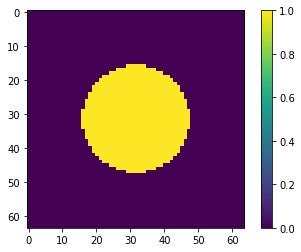
\includegraphics[width=0.32\textwidth]{../Common_Images/lifted/Numerical_Perceptron_circle_image.png}
    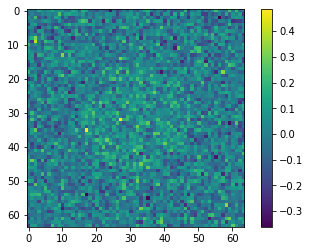
\includegraphics[width=0.32\textwidth]{../Common_Images/lifted/Numerical_Perceptron_Circle_Landweber_Regularisation.png}
    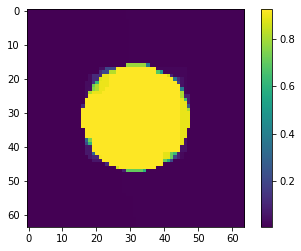
\includegraphics[width=0.32\textwidth]{../Common_Images/lifted/Numerical_Perceptron_Circle_TV_Regularisation.png}
    \caption{Perceptron inversion toy example (adapted from \cite{wang2023inversion}). Left: ground-truth circle. Middle: Landweber-type reconstruction. Right: lifted Bregman inversion with TV regularisation, showing a substantially more meaningful structure.}
    \label{fig:perceptron_inversion_circle_comparison_ch9}
\end{figure}

The authors of \cite{wang2023inversion} also report MNIST-based perceptron inversion examples; a representative validation visualisation is shown in Figure~\ref{fig:perceptron_mnist_inversion_validation_ch9}. Here the comparison is between the lifted inverse reconstructions and decoder-style baseline inversions for the same perturbed outputs.
\begin{figure}[ht]
    \centering
    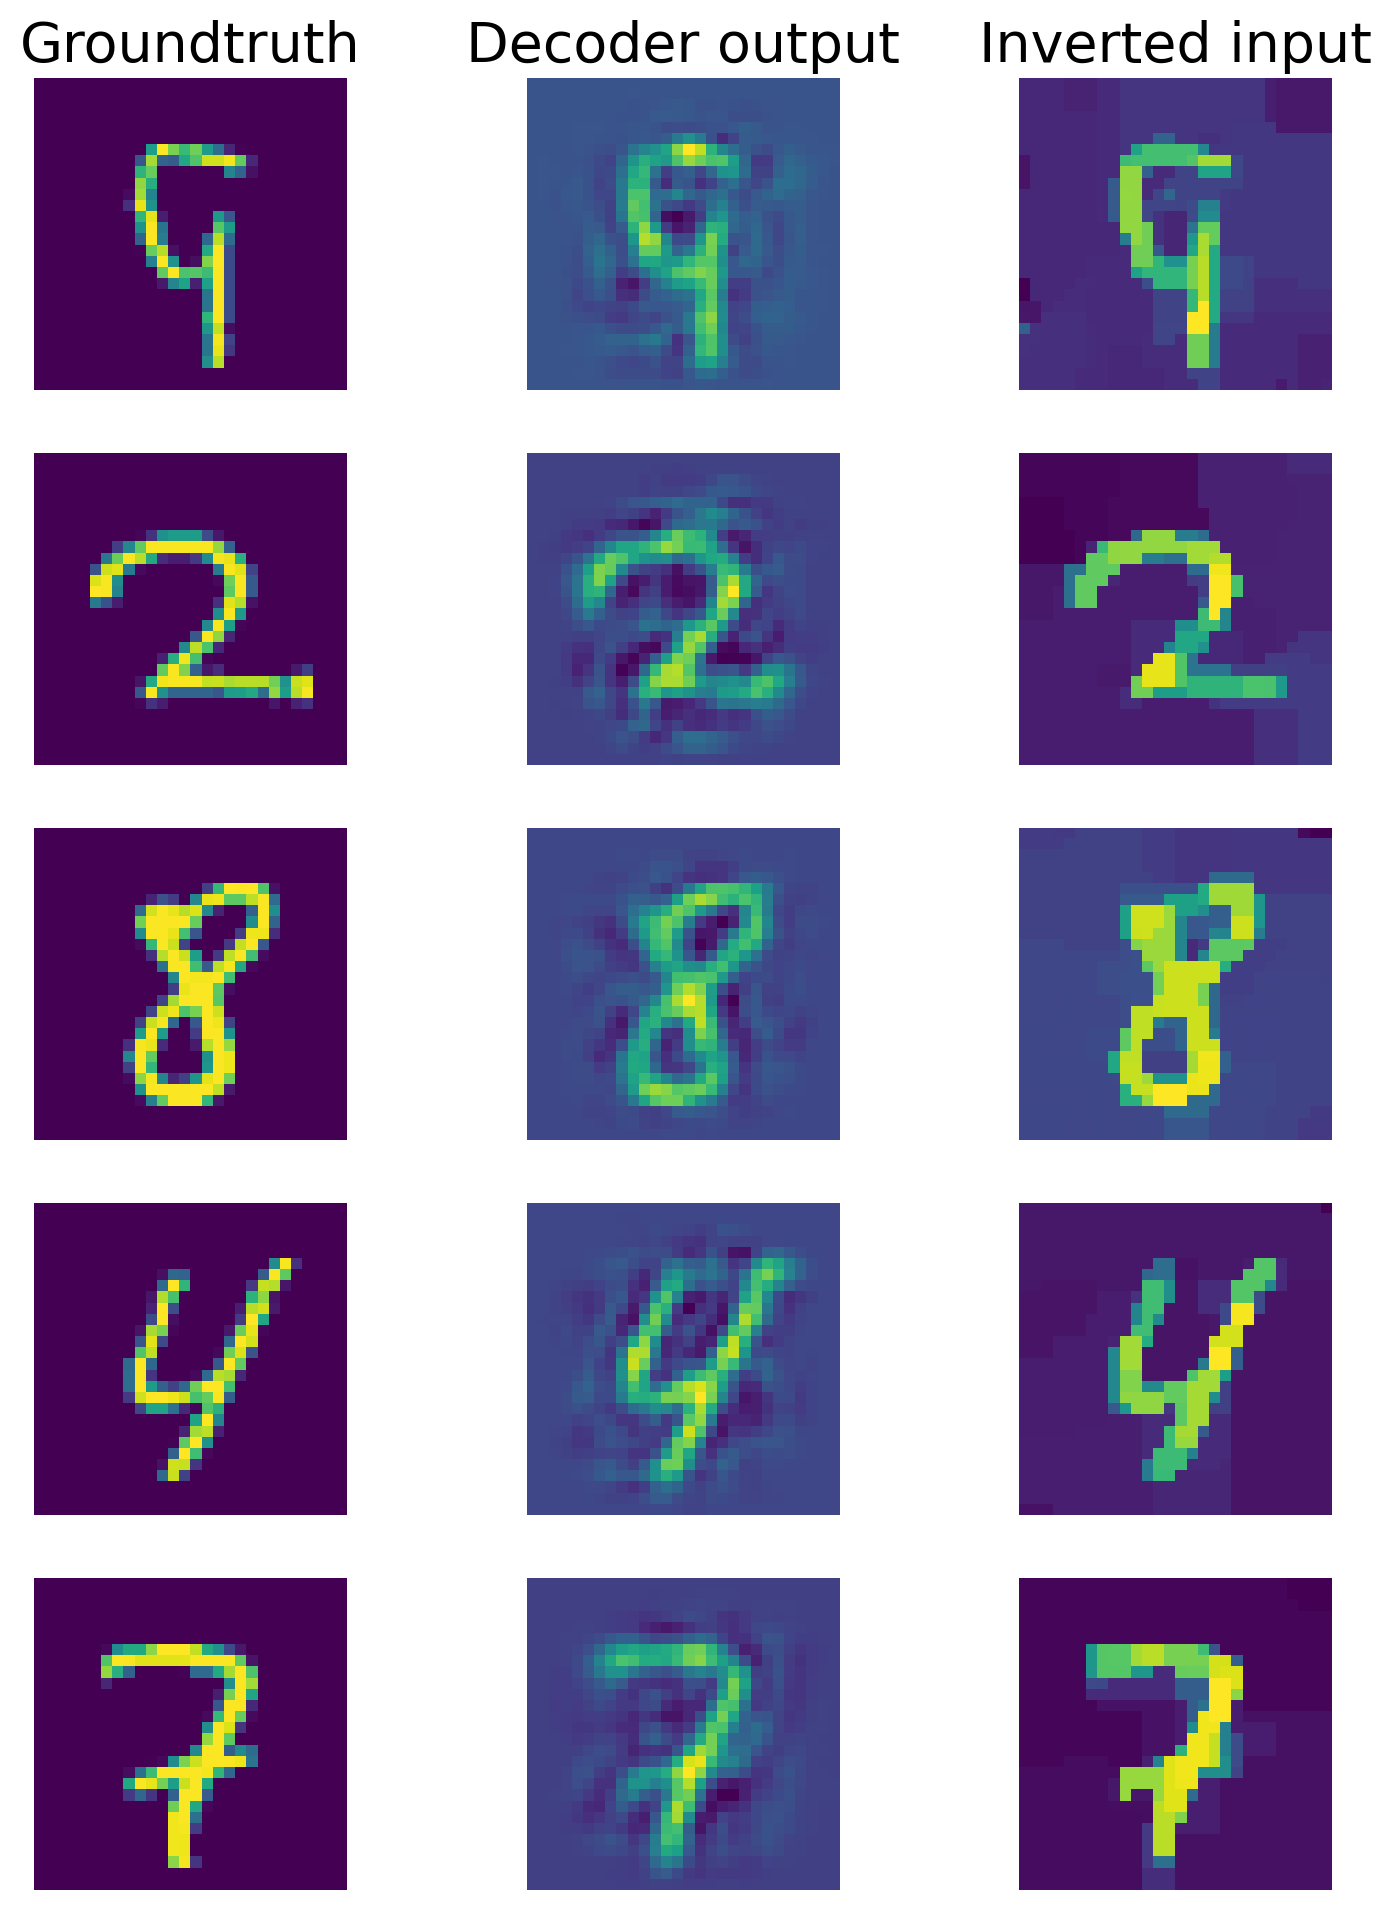
\includegraphics[width=0.9\textwidth]{../Common_Images/lifted/Numerical_Perceptron_Inversion_MNIST_Val_Samples.png}
    \caption{Perceptron inversion on MNIST validation samples (adapted from \cite{wang2023inversion}). The lifted model-based inversion remains visually robust under output perturbations and compares favourably to direct decoder-style baselines.}
    \label{fig:perceptron_mnist_inversion_validation_ch9}
\end{figure}

From the unified framework chapter \cite{wang2025unified}, we further include multi-layer autoencoder inversion under noisy latent observations. The experiment uses a six-layer MNIST autoencoder: the encoder consists of two convolutional ReLU layers that reduce the spatial resolution from $28\times 28$ to $14\times 14$ and then to $7\times 7$ while increasing the channel count from $1$ to $8$ and $16$, followed by a fully connected layer mapping to a $392$-dimensional latent code. The decoder mirrors this with one fully connected ReLU layer and two transposed-convolution layers to return to image space. After training the autoencoder by MSE minimisation, the inversion experiment perturbs the encoder output by Gaussian noise and reconstructs the input from this noisy latent observation via the BCD+PDHG strategy above, with PDHG stopping by primal/dual increments and an outer coordinate-descent cap.

The comparison in Figure~\ref{fig:mlp_inversion_unified_ch9} is therefore explicit: row 1 is the ground-truth MNIST input, row 2 is the ordinary autoencoder reconstruction produced by a forward pass through the trained network, and row 3 is the lifted inversion result obtained by solving the variational inverse problem from the noisy encoder code. This separates decoder quality from inversion quality.
\begin{figure}[ht]
    \centering
    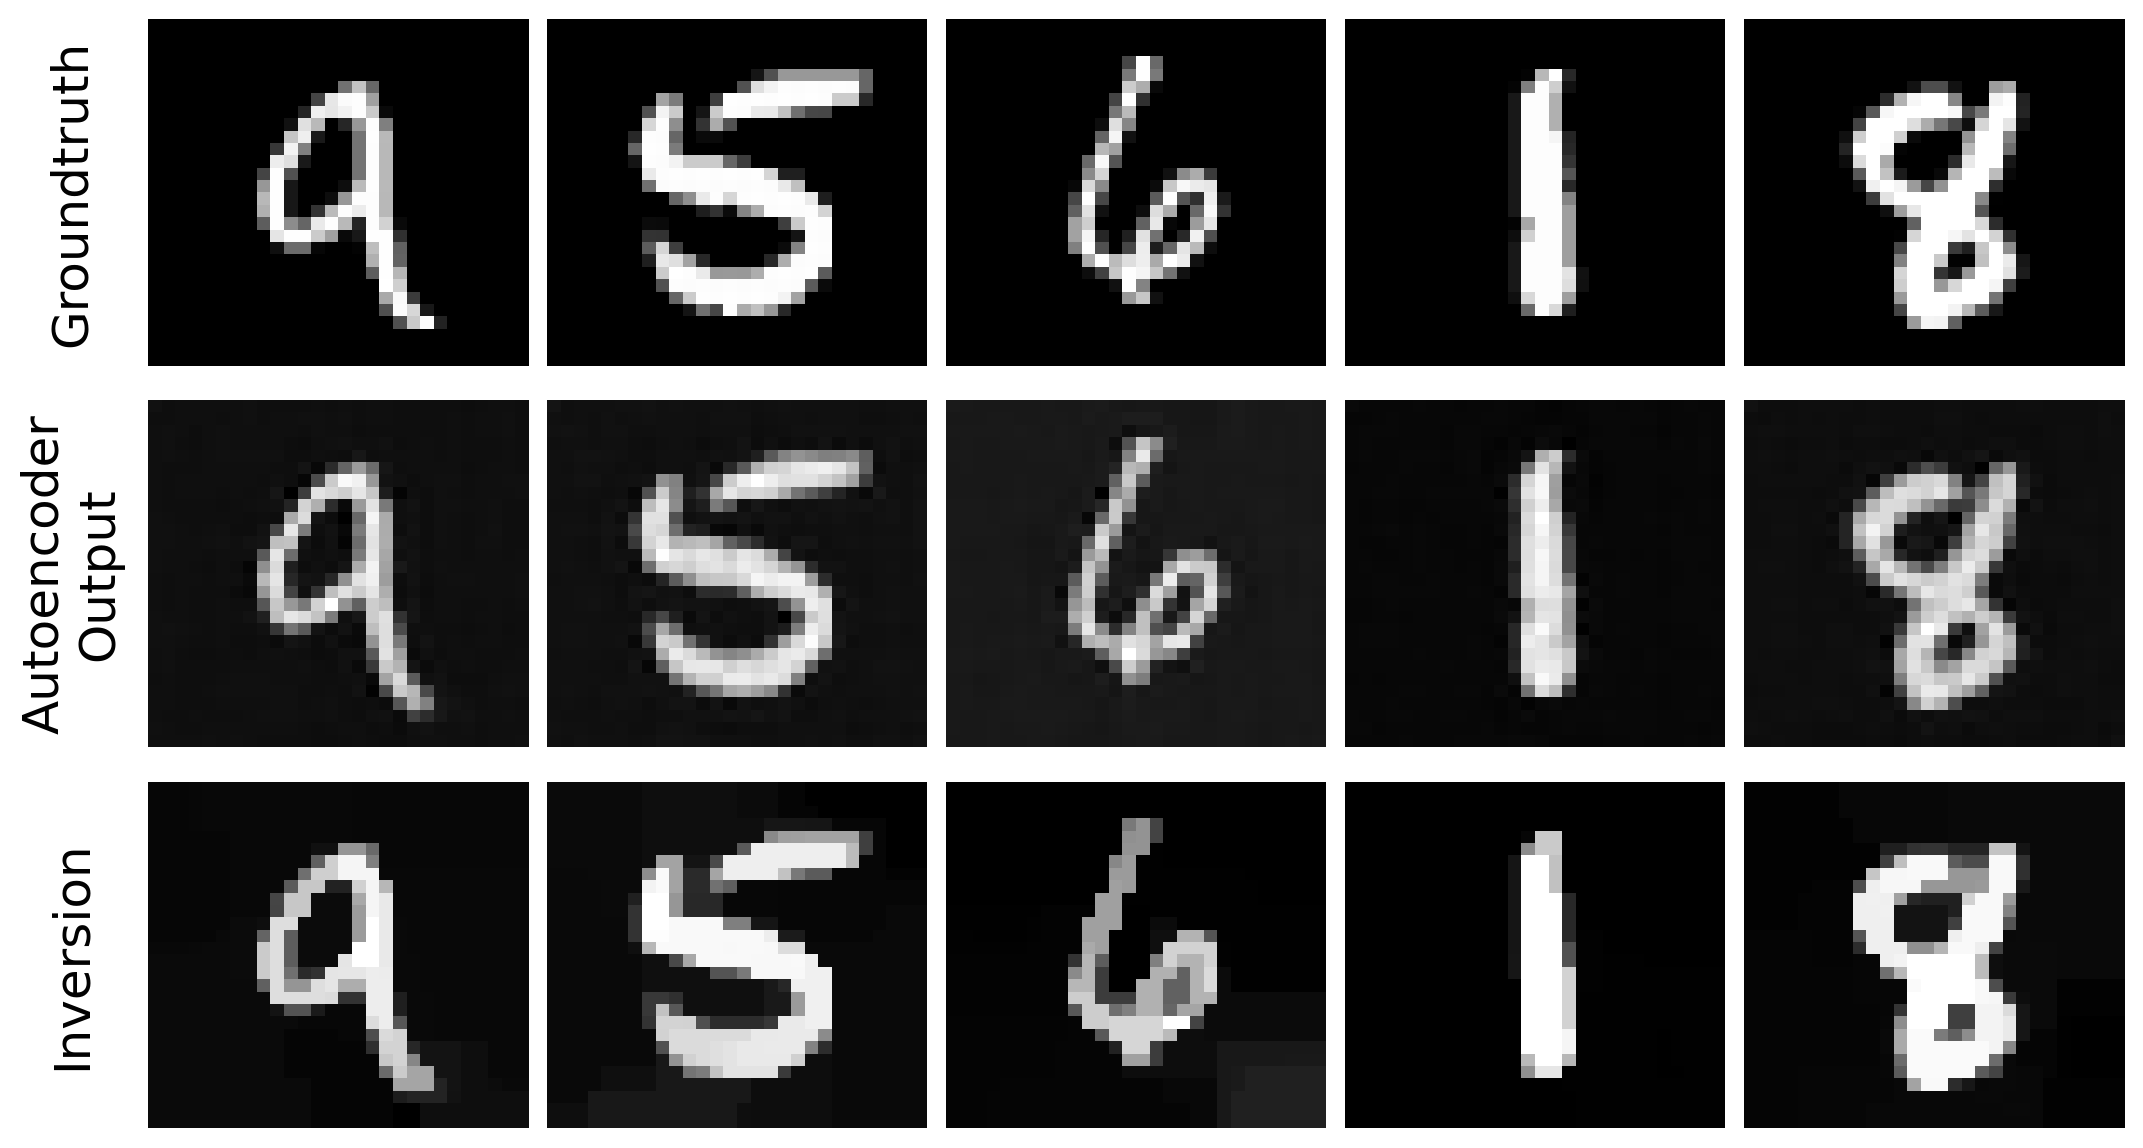
\includegraphics[width=0.9\textwidth]{../Common_Images/lifted/mlp_inversion_gray.png}
    \caption{Multi-layer autoencoder inversion on MNIST (adapted from \cite{wang2025unified}). Row 1: ground-truth inputs. Row 2: standard autoencoder reconstructions obtained by a forward pass through the trained decoder. Row 3: lifted inversion reconstructions recovered from noisy encoder measurements.}
    \label{fig:mlp_inversion_unified_ch9}
\end{figure}

To highlight dependence on network quality, Figures~\ref{fig:mlp_inversion_undertrained_severe_ch9} and \ref{fig:mlp_inversion_undertrained_moderate_ch9} show the same inversion procedure applied to severely and moderately under-trained autoencoders. The point of this comparison is not merely visual: it shows how the quality of the trained forward model affects both the ordinary decoder output and the lifted inverse, while still indicating that the inversion framework recovers approximate digit structure even when the network itself is not fully trained.
\begin{figure}[ht]
    \centering
    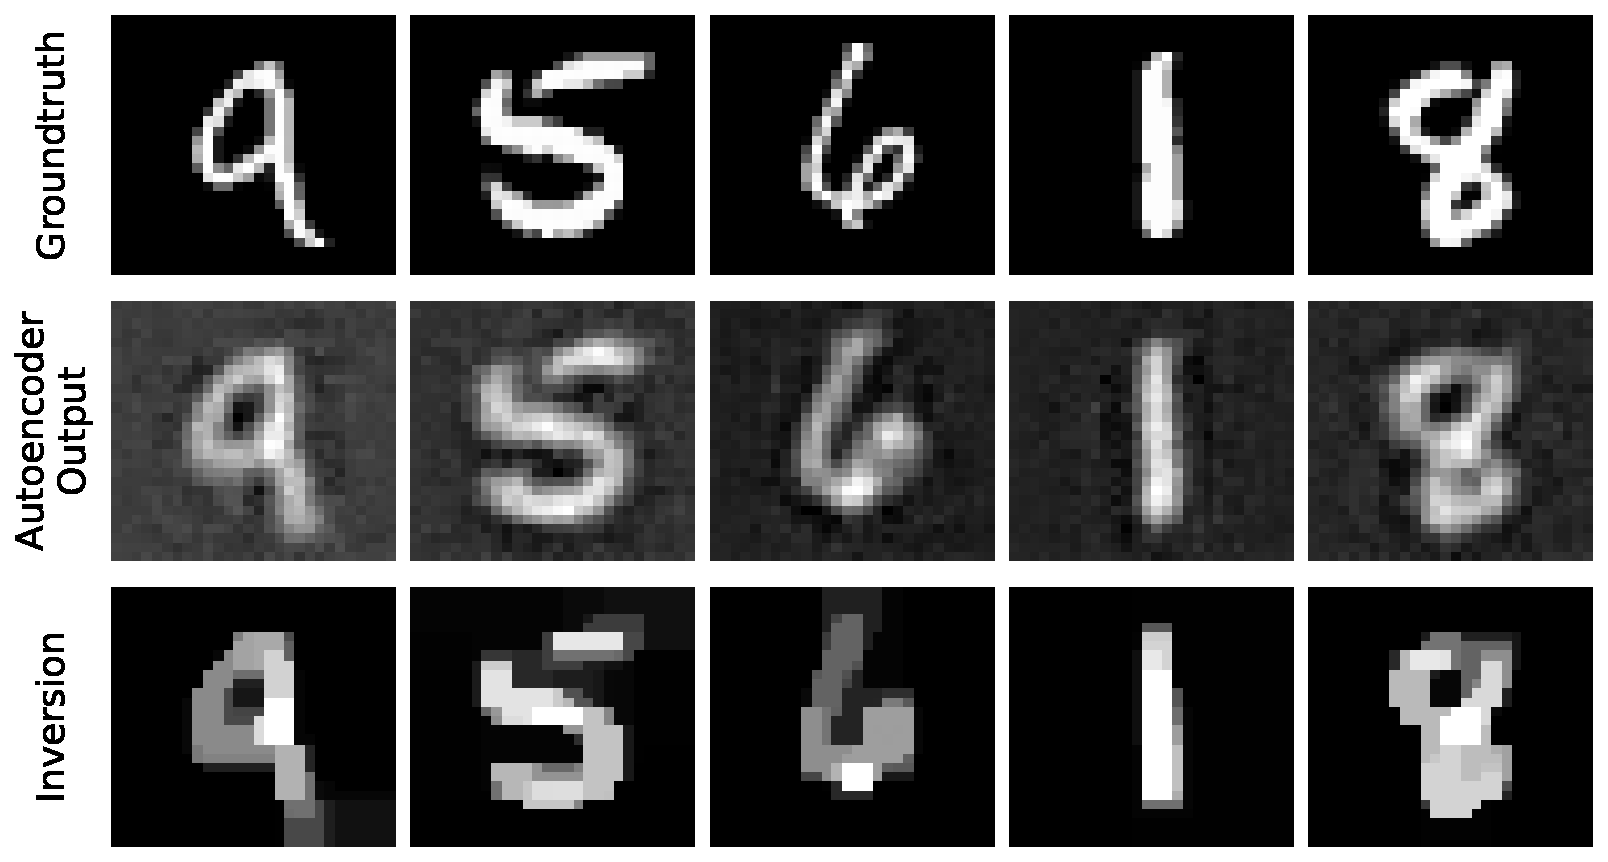
\includegraphics[width=0.85\textwidth]{../Common_Images/lifted/mlp_inv_su.pdf}
    \caption{Lifted inversion with a severely under-trained autoencoder (adapted from \cite{wang2025unified}). As in Figure~\ref{fig:mlp_inversion_unified_ch9}, the comparison is between ground truth, the ordinary decoder output, and the lifted inverse; the inversion still returns approximate digit structure, but with visibly degraded quality compared to the near-converged network.}
    \label{fig:mlp_inversion_undertrained_severe_ch9}
\end{figure}

\begin{figure}[ht]
    \centering
    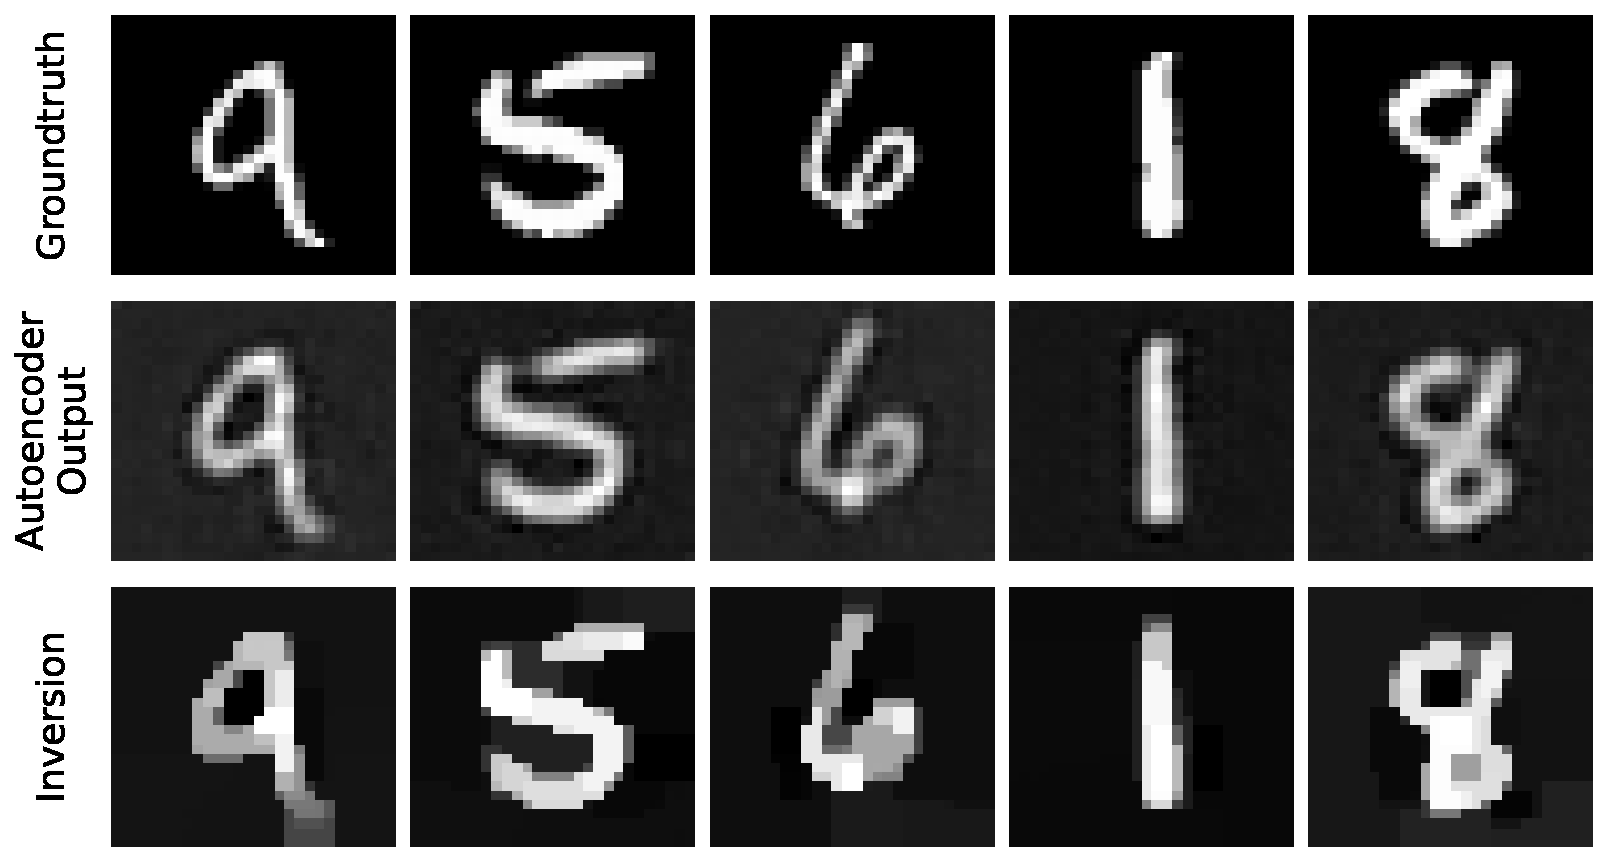
\includegraphics[width=0.85\textwidth]{../Common_Images/lifted/mlp_inv_u.pdf}
    \caption{Lifted inversion with a moderately under-trained autoencoder (adapted from \cite{wang2025unified}). Again comparing ground truth, ordinary decoder output, and lifted inverse, the quality improves over the severely under-trained case and approaches the near-converged baseline as training loss decreases.}
    \label{fig:mlp_inversion_undertrained_moderate_ch9}
\end{figure}

% Finally, for training-based inverse imaging tasks, \cite{wang2025unified} reports PSNR evolution for deblurring under lifted versus conventional training. This supports the same background message: proximal-structured lifted optimisation can improve stability/generalisation under stronger regularisation.
% \begin{figure}[ht]
%     \centering
%     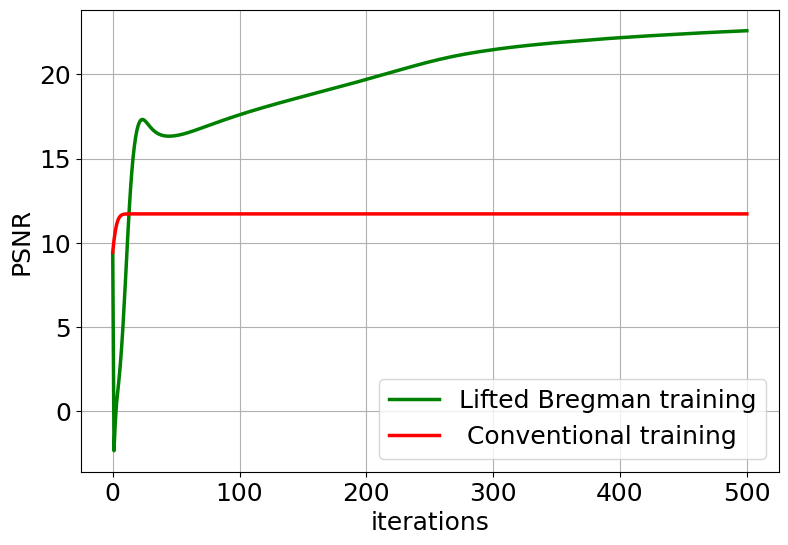
\includegraphics[width=0.7\textwidth]{../Common_Images/lifted/deblurring_psnr_comparison.png}
%     \caption{Deblurring PSNR comparison from \cite{wang2025unified}. Lifted Bregman training maintains stronger reconstruction quality across training iterations, especially in higher-shrinkage settings.}
%     \label{fig:deblurring_psnr_unified_ch9}
% \end{figure}
